% Options for packages loaded elsewhere
% Options for packages loaded elsewhere
\PassOptionsToPackage{unicode}{hyperref}
\PassOptionsToPackage{hyphens}{url}
\PassOptionsToPackage{dvipsnames,svgnames,x11names}{xcolor}
%
\documentclass[
  letterpaper,
  DIV=11,
  numbers=noendperiod]{scrartcl}
\usepackage{xcolor}
\usepackage[margin=1in]{geometry}
\usepackage{amsmath,amssymb}
\setcounter{secnumdepth}{5}
\usepackage{iftex}
\ifPDFTeX
  \usepackage[T1]{fontenc}
  \usepackage[utf8]{inputenc}
  \usepackage{textcomp} % provide euro and other symbols
\else % if luatex or xetex
  \usepackage{unicode-math} % this also loads fontspec
  \defaultfontfeatures{Scale=MatchLowercase}
  \defaultfontfeatures[\rmfamily]{Ligatures=TeX,Scale=1}
\fi
\usepackage{lmodern}
\ifPDFTeX\else
  % xetex/luatex font selection
  \setmainfont[]{Latin Modern Roman}
  \setsansfont[]{Latin Modern Sans}
  \setmonofont[]{Latin Modern Mono}
\fi
% Use upquote if available, for straight quotes in verbatim environments
\IfFileExists{upquote.sty}{\usepackage{upquote}}{}
\IfFileExists{microtype.sty}{% use microtype if available
  \usepackage[]{microtype}
  \UseMicrotypeSet[protrusion]{basicmath} % disable protrusion for tt fonts
}{}
\makeatletter
\@ifundefined{KOMAClassName}{% if non-KOMA class
  \IfFileExists{parskip.sty}{%
    \usepackage{parskip}
  }{% else
    \setlength{\parindent}{0pt}
    \setlength{\parskip}{6pt plus 2pt minus 1pt}}
}{% if KOMA class
  \KOMAoptions{parskip=half}}
\makeatother
% Make \paragraph and \subparagraph free-standing
\makeatletter
\ifx\paragraph\undefined\else
  \let\oldparagraph\paragraph
  \renewcommand{\paragraph}{
    \@ifstar
      \xxxParagraphStar
      \xxxParagraphNoStar
  }
  \newcommand{\xxxParagraphStar}[1]{\oldparagraph*{#1}\mbox{}}
  \newcommand{\xxxParagraphNoStar}[1]{\oldparagraph{#1}\mbox{}}
\fi
\ifx\subparagraph\undefined\else
  \let\oldsubparagraph\subparagraph
  \renewcommand{\subparagraph}{
    \@ifstar
      \xxxSubParagraphStar
      \xxxSubParagraphNoStar
  }
  \newcommand{\xxxSubParagraphStar}[1]{\oldsubparagraph*{#1}\mbox{}}
  \newcommand{\xxxSubParagraphNoStar}[1]{\oldsubparagraph{#1}\mbox{}}
\fi
\makeatother

\usepackage{color}
\usepackage{fancyvrb}
\newcommand{\VerbBar}{|}
\newcommand{\VERB}{\Verb[commandchars=\\\{\}]}
\DefineVerbatimEnvironment{Highlighting}{Verbatim}{commandchars=\\\{\}}
% Add ',fontsize=\small' for more characters per line
\usepackage{framed}
\definecolor{shadecolor}{RGB}{241,243,245}
\newenvironment{Shaded}{\begin{snugshade}}{\end{snugshade}}
\newcommand{\AlertTok}[1]{\textcolor[rgb]{0.68,0.00,0.00}{#1}}
\newcommand{\AnnotationTok}[1]{\textcolor[rgb]{0.37,0.37,0.37}{#1}}
\newcommand{\AttributeTok}[1]{\textcolor[rgb]{0.40,0.45,0.13}{#1}}
\newcommand{\BaseNTok}[1]{\textcolor[rgb]{0.68,0.00,0.00}{#1}}
\newcommand{\BuiltInTok}[1]{\textcolor[rgb]{0.00,0.23,0.31}{#1}}
\newcommand{\CharTok}[1]{\textcolor[rgb]{0.13,0.47,0.30}{#1}}
\newcommand{\CommentTok}[1]{\textcolor[rgb]{0.37,0.37,0.37}{#1}}
\newcommand{\CommentVarTok}[1]{\textcolor[rgb]{0.37,0.37,0.37}{\textit{#1}}}
\newcommand{\ConstantTok}[1]{\textcolor[rgb]{0.56,0.35,0.01}{#1}}
\newcommand{\ControlFlowTok}[1]{\textcolor[rgb]{0.00,0.23,0.31}{\textbf{#1}}}
\newcommand{\DataTypeTok}[1]{\textcolor[rgb]{0.68,0.00,0.00}{#1}}
\newcommand{\DecValTok}[1]{\textcolor[rgb]{0.68,0.00,0.00}{#1}}
\newcommand{\DocumentationTok}[1]{\textcolor[rgb]{0.37,0.37,0.37}{\textit{#1}}}
\newcommand{\ErrorTok}[1]{\textcolor[rgb]{0.68,0.00,0.00}{#1}}
\newcommand{\ExtensionTok}[1]{\textcolor[rgb]{0.00,0.23,0.31}{#1}}
\newcommand{\FloatTok}[1]{\textcolor[rgb]{0.68,0.00,0.00}{#1}}
\newcommand{\FunctionTok}[1]{\textcolor[rgb]{0.28,0.35,0.67}{#1}}
\newcommand{\ImportTok}[1]{\textcolor[rgb]{0.00,0.46,0.62}{#1}}
\newcommand{\InformationTok}[1]{\textcolor[rgb]{0.37,0.37,0.37}{#1}}
\newcommand{\KeywordTok}[1]{\textcolor[rgb]{0.00,0.23,0.31}{\textbf{#1}}}
\newcommand{\NormalTok}[1]{\textcolor[rgb]{0.00,0.23,0.31}{#1}}
\newcommand{\OperatorTok}[1]{\textcolor[rgb]{0.37,0.37,0.37}{#1}}
\newcommand{\OtherTok}[1]{\textcolor[rgb]{0.00,0.23,0.31}{#1}}
\newcommand{\PreprocessorTok}[1]{\textcolor[rgb]{0.68,0.00,0.00}{#1}}
\newcommand{\RegionMarkerTok}[1]{\textcolor[rgb]{0.00,0.23,0.31}{#1}}
\newcommand{\SpecialCharTok}[1]{\textcolor[rgb]{0.37,0.37,0.37}{#1}}
\newcommand{\SpecialStringTok}[1]{\textcolor[rgb]{0.13,0.47,0.30}{#1}}
\newcommand{\StringTok}[1]{\textcolor[rgb]{0.13,0.47,0.30}{#1}}
\newcommand{\VariableTok}[1]{\textcolor[rgb]{0.07,0.07,0.07}{#1}}
\newcommand{\VerbatimStringTok}[1]{\textcolor[rgb]{0.13,0.47,0.30}{#1}}
\newcommand{\WarningTok}[1]{\textcolor[rgb]{0.37,0.37,0.37}{\textit{#1}}}

\usepackage{longtable,booktabs,array}
\usepackage{calc} % for calculating minipage widths
% Correct order of tables after \paragraph or \subparagraph
\usepackage{etoolbox}
\makeatletter
\patchcmd\longtable{\par}{\if@noskipsec\mbox{}\fi\par}{}{}
\makeatother
% Allow footnotes in longtable head/foot
\IfFileExists{footnotehyper.sty}{\usepackage{footnotehyper}}{\usepackage{footnote}}
\makesavenoteenv{longtable}
\usepackage{graphicx}
\makeatletter
\newsavebox\pandoc@box
\newcommand*\pandocbounded[1]{% scales image to fit in text height/width
  \sbox\pandoc@box{#1}%
  \Gscale@div\@tempa{\textheight}{\dimexpr\ht\pandoc@box+\dp\pandoc@box\relax}%
  \Gscale@div\@tempb{\linewidth}{\wd\pandoc@box}%
  \ifdim\@tempb\p@<\@tempa\p@\let\@tempa\@tempb\fi% select the smaller of both
  \ifdim\@tempa\p@<\p@\scalebox{\@tempa}{\usebox\pandoc@box}%
  \else\usebox{\pandoc@box}%
  \fi%
}
% Set default figure placement to htbp
\def\fps@figure{htbp}
\makeatother





\setlength{\emergencystretch}{3em} % prevent overfull lines

\providecommand{\tightlist}{%
  \setlength{\itemsep}{0pt}\setlength{\parskip}{0pt}}



 


% Colors and section/title styling using KOMA-Script interfaces
\usepackage{xcolor}
\definecolor{sectionblue}{HTML}{2563eb}

% KOMA: headings and title/subtitle colors
\setkomafont{title}{\color{sectionblue}\bfseries\Huge}
\setkomafont{subtitle}{\color{sectionblue}\large}
\setkomafont{section}{\color{sectionblue}\bfseries\Large}
\setkomafont{subsection}{\color{sectionblue}\bfseries\large}

% Code block styling via Shaded redefinition
\usepackage{tcolorbox}
\tcbuselibrary{skins,breakable}
\definecolor{codebg}{HTML}{F0F8FF}
\renewenvironment{Shaded}{%
  \begin{tcolorbox}[%
    enhanced,%
    colback=codebg,%
    colframe=codebg,%
    borderline west={3pt}{0pt}{sectionblue},%
    boxrule=0pt,%
    arc=0pt,%
    boxsep=5pt,%
    left=2mm,%
    right=2mm,%
    top=2mm,%
    bottom=2mm% 
  ]% 
}{%
  \end{tcolorbox}%
}
\KOMAoption{captions}{tableheading}
\makeatletter
\@ifpackageloaded{caption}{}{\usepackage{caption}}
\AtBeginDocument{%
\ifdefined\contentsname
  \renewcommand*\contentsname{Table of contents}
\else
  \newcommand\contentsname{Table of contents}
\fi
\ifdefined\listfigurename
  \renewcommand*\listfigurename{List of Figures}
\else
  \newcommand\listfigurename{List of Figures}
\fi
\ifdefined\listtablename
  \renewcommand*\listtablename{List of Tables}
\else
  \newcommand\listtablename{List of Tables}
\fi
\ifdefined\figurename
  \renewcommand*\figurename{Figure}
\else
  \newcommand\figurename{Figure}
\fi
\ifdefined\tablename
  \renewcommand*\tablename{Table}
\else
  \newcommand\tablename{Table}
\fi
}
\@ifpackageloaded{float}{}{\usepackage{float}}
\floatstyle{ruled}
\@ifundefined{c@chapter}{\newfloat{codelisting}{h}{lop}}{\newfloat{codelisting}{h}{lop}[chapter]}
\floatname{codelisting}{Listing}
\newcommand*\listoflistings{\listof{codelisting}{List of Listings}}
\makeatother
\makeatletter
\makeatother
\makeatletter
\@ifpackageloaded{caption}{}{\usepackage{caption}}
\@ifpackageloaded{subcaption}{}{\usepackage{subcaption}}
\makeatother
\makeatletter
\definecolor{QuartoInternalColor6}{rgb}{0.00,0.00,1.00}
\definecolor{QuartoInternalColor4}{rgb}{0.00,0.64,0.31}
\definecolor{QuartoInternalColor7}{rgb}{0.38,0.38,0.38}
\definecolor{QuartoInternalColor10}{rgb}{0.00,0.40,0.79}
\definecolor{QuartoInternalColor3}{rgb}{0.00,0.45,0.15}
\definecolor{QuartoInternalColor5}{rgb}{0.00,0.40,0.00}
\definecolor{QuartoInternalColor2}{rgb}{0,0,0}
\definecolor{QuartoInternalColor8}{rgb}{0.60,0.00,0.00}
\definecolor{QuartoInternalColor11}{rgb}{0.74,0.74,0.74}
\definecolor{QuartoInternalColor1}{rgb}{0.70,0.17,0.19}
\definecolor{QuartoInternalColor9}{rgb}{0.15,0.56,0.56}
\makeatother
\usepackage{bookmark}
\IfFileExists{xurl.sty}{\usepackage{xurl}}{} % add URL line breaks if available
\urlstyle{same}
\hypersetup{
  pdftitle={Fine-Grained Dog Breed Classification: A Deep Learning Approach},
  colorlinks=true,
  linkcolor={blue},
  filecolor={Maroon},
  citecolor={Blue},
  urlcolor={Blue},
  pdfcreator={LaTeX via pandoc}}


\title{Fine-Grained Dog Breed Classification: A Deep Learning Approach}
\usepackage{etoolbox}
\makeatletter
\providecommand{\subtitle}[1]{% add subtitle to \maketitle
  \apptocmd{\@title}{\par {\large #1 \par}}{}{}
}
\makeatother
\subtitle{Building State-of-the-Art CNN Models for 120-Class Visual
Recognition}
\author{}
\date{}
\begin{document}
\maketitle

\renewcommand*\contentsname{Table of contents}
{
\hypersetup{linkcolor=}
\setcounter{tocdepth}{3}
\tableofcontents
}

\section{Project Introduction}\label{project-introduction}

\subsection{What This Project Is
About}\label{what-this-project-is-about}

This project tackles the problem of \textbf{fine-grained image
classification} using \textbf{Convolutional Neural Networks (CNNs)}.
Specifically, I will build a deep learning model to classify images of
dogs into their specific breeds. This is a \textbf{multi-class
classification problem} with 120 different dog breed categories.

The architecture approach will utilize \textbf{transfer learning with
pre-trained CNN models} trained on ImageNet. I will implement and
compare multiple architectures:

\begin{enumerate}
\def\labelenumi{\arabic{enumi}.}
\tightlist
\item
  \textbf{Transfer Learning Approach}: Use pre-trained models (ResNet50,
  VGG16, or EfficientNetB0) as feature extractors, freeze the
  convolutional base, and train only the new fully connected
  classification layers on the dog breed dataset
\item
  \textbf{Fine-Tuning Approach}: Start with pre-trained weights, then
  unfreeze some of the top convolutional layers and fine-tune them along
  with the classification layers using a low learning rate
\item
  \textbf{Custom CNN Architecture}: Build a CNN from scratch with
  multiple convolutional blocks (Conv2D + BatchNormalization +
  MaxPooling + Dropout) to serve as a baseline for comparison
\end{enumerate}

I will compare these approaches to determine which strategy yields the
best performance for this specific classification task.

\subsection{Goal and Motivation}\label{goal-and-motivation}

\textbf{Goal}: To develop an accurate deep learning classifier that can
identify dog breeds from images with high precision, and to understand
which architectural approach works best for fine-grained visual
recognition.

\textbf{Why This Matters}:

\begin{itemize}
\tightlist
\item
  \textbf{Practical Application}: Automated breed identification can
  help in animal shelters, veterinary clinics, and pet adoption services
  where quick and accurate breed identification is essential
\item
  \textbf{Lost Pet Recovery}: Can assist in matching found dogs with
  lost pet reports
\item
  \textbf{Education}: Helps dog enthusiasts and potential pet owners
  learn about different breeds
\item
  \textbf{Technical Challenge}: Dog breed classification is a
  challenging fine-grained visual recognition problem because many
  breeds share similar physical characteristics (facial features, body
  shape, coat patterns), making it an excellent testbed for evaluating
  deep learning techniques and transfer learning strategies
\end{itemize}

\textbf{What I Want to Achieve}:

\begin{itemize}
\tightlist
\item
  Build a model that can accurately distinguish between 120 dog breeds,
  even when breeds look visually similar (e.g., Siberian Husky
  vs.~Alaskan Malamute)
\item
  Compare the effectiveness of transfer learning versus training from
  scratch
\item
  Understand which visual features the model uses to make distinctions
  through visualization techniques (such as class activation maps)
\item
  Achieve practical accuracy that could be deployed in real-world
  applications
\end{itemize}

\begin{center}\rule{0.5\linewidth}{0.5pt}\end{center}

\textbf{Expected Outcomes}: A trained CNN model with \textgreater80\%
accuracy on the test set, comprehensive comparison of different
architectures, and insights into what makes certain breeds easier or
harder to classify.

\section{Data Loading \& Initial
Inspection}\label{data-loading-initial-inspection}

\subsection{Dataset: Stanford Dogs}\label{dataset-stanford-dogs}

\textbf{Source}: Stanford Dogs Dataset\\
\textbf{URL}: http://vision.stanford.edu/aditya86/ImageNetDogs/\\
\textbf{License}: Academic/Research use\\
\textbf{Size}: \textasciitilde750MB (images), 20,580 total images

\textbf{Dataset Description}:

The Stanford Dogs dataset contains images of 120 breeds of dogs from
around the world. This dataset has been built using images and
annotation from ImageNet for the task of fine-grained image
categorization.

\textbf{Key Statistics}:

\begin{itemize}
\tightlist
\item
  \textbf{120 dog breed classes} (Chihuahua, Afghan\_hound,
  Maltese\_dog, Golden\_retriever, etc.)
\item
  \textbf{20,580 images total} (after validation)
\item
  \textbf{Average 171.5 images per breed} (range: 148-252)
\item
  \textbf{Average image dimensions}: 443×386 pixels
\item
  \textbf{Image format}: JPEG (20,579 images), PNG (1 image)
\item
  \textbf{Color mode}: RGB (20,579 images), RGBA (1 image)
\end{itemize}

\textbf{Data Organization}:

Images are organized in directories by breed:

\begin{verbatim}
data/raw/Images/
├── n02085620-Chihuahua/
├── n02085782-Japanese_spaniel/
├── n02085936-Maltese_dog/
└── ... (120 breed directories total)
\end{verbatim}

\textbf{Preprocessing Pipeline}:

\begin{enumerate}
\def\labelenumi{\arabic{enumi}.}
\tightlist
\item
  \textbf{Download} (\texttt{python\ -m\ dbc.ingest}): Downloaded
  images, annotations, and breed mapping
\item
  \textbf{Validation} (\texttt{python\ -m\ dbc.preprocess}): Scanned all
  20,580 images, validated for corruption, size, and format
\item
  \textbf{Cleaning}: Removed 0 corrupt images, all images passed
  validation ✓
\item
  \textbf{Splitting}: Created stratified 80/20 train/validation split

  \begin{itemize}
  \tightlist
  \item
    Train: 16,508 images
  \item
    Validation: 4,072 images
  \end{itemize}
\end{enumerate}

\textbf{Why This Dataset?}:

\begin{itemize}
\tightlist
\item
  \textbf{Fine-grained classification challenge}: Many breeds share
  similar visual features, making this an excellent test for CNN
  architectures
\item
  \textbf{Sufficient data}: \textasciitilde170 images per class enables
  meaningful training with data augmentation
\item
  \textbf{Real-world applicability}: Breed identification has practical
  uses in animal shelters, veterinary clinics, and pet services
\end{itemize}

\textbf{Dataset Challenges}:

This dataset presents several real-world complications that make
classification more challenging:

\begin{itemize}
\tightlist
\item
  \textbf{Multiple Objects}: Many images contain humans, other animals,
  or various background objects alongside the dogs
\item
  \textbf{Variable Composition}: Dogs may occupy only a small portion of
  the image frame
\item
  \textbf{Background Clutter}: Complex backgrounds with furniture,
  outdoor scenery, or other distractions
\item
  \textbf{Occlusion}: Dogs may be partially hidden or cropped in some
  images
\end{itemize}

These challenges make the task more realistic and require the model to
learn discriminative breed features despite visual noise.

\begin{Shaded}
\begin{Highlighting}[]
\ImportTok{import}\NormalTok{ sys}
\ImportTok{from}\NormalTok{ pathlib }\ImportTok{import}\NormalTok{ Path}
\NormalTok{sys.path.append(}\BuiltInTok{str}\NormalTok{(Path.cwd().parent }\OperatorTok{/} \StringTok{"src"}\NormalTok{))}

\ImportTok{import}\NormalTok{ pandas }\ImportTok{as}\NormalTok{ pd}
\ImportTok{import}\NormalTok{ numpy }\ImportTok{as}\NormalTok{ np}
\ImportTok{import}\NormalTok{ matplotlib.pyplot }\ImportTok{as}\NormalTok{ plt}
\ImportTok{from}\NormalTok{ PIL }\ImportTok{import}\NormalTok{ Image}
\ImportTok{from}\NormalTok{ IPython.display }\ImportTok{import}\NormalTok{ display}
\ImportTok{import}\NormalTok{ json}

\CommentTok{\# Load breed mapping}
\NormalTok{breeds\_df }\OperatorTok{=}\NormalTok{ pd.read\_csv(}\StringTok{"../data/raw/breed\_mapping.csv"}\NormalTok{)}
\BuiltInTok{print}\NormalTok{(}\StringTok{"Breed Mapping (first 10 breeds):"}\NormalTok{)}
\NormalTok{display(breeds\_df.head(}\DecValTok{10}\NormalTok{))}

\CommentTok{\# Load train/val metadata}
\NormalTok{train\_df }\OperatorTok{=}\NormalTok{ pd.read\_csv(}\StringTok{"../artifacts/train\_metadata.csv"}\NormalTok{)}
\NormalTok{val\_df }\OperatorTok{=}\NormalTok{ pd.read\_csv(}\StringTok{"../artifacts/val\_metadata.csv"}\NormalTok{)}

\BuiltInTok{print}\NormalTok{(}\SpecialStringTok{f"}\CharTok{\textbackslash{}n}\SpecialStringTok{Train set: }\SpecialCharTok{\{}\BuiltInTok{len}\NormalTok{(train\_df)}\SpecialCharTok{\}}\SpecialStringTok{ images"}\NormalTok{)}
\BuiltInTok{print}\NormalTok{(}\SpecialStringTok{f"Validation set: }\SpecialCharTok{\{}\BuiltInTok{len}\NormalTok{(val\_df)}\SpecialCharTok{\}}\SpecialStringTok{ images"}\NormalTok{)}

\CommentTok{\# Load dataset statistics}
\ControlFlowTok{with} \BuiltInTok{open}\NormalTok{(}\StringTok{"../artifacts/dataset\_stats.json"}\NormalTok{, }\StringTok{"r"}\NormalTok{) }\ImportTok{as}\NormalTok{ f:}
\NormalTok{    stats }\OperatorTok{=}\NormalTok{ json.load(f)}
    
\BuiltInTok{print}\NormalTok{(}\StringTok{"}\CharTok{\textbackslash{}n}\StringTok{Dataset Statistics:"}\NormalTok{)}
\ControlFlowTok{for}\NormalTok{ key, value }\KeywordTok{in}\NormalTok{ stats.items():}
    \ControlFlowTok{if}\NormalTok{ key }\KeywordTok{not} \KeywordTok{in}\NormalTok{ [}\StringTok{\textquotesingle{}image\_modes\textquotesingle{}}\NormalTok{, }\StringTok{\textquotesingle{}image\_formats\textquotesingle{}}\NormalTok{]:}
        \BuiltInTok{print}\NormalTok{(}\SpecialStringTok{f"  }\SpecialCharTok{\{}\NormalTok{key}\SpecialCharTok{\}}\SpecialStringTok{: }\SpecialCharTok{\{}\NormalTok{value}\SpecialCharTok{\}}\SpecialStringTok{"}\NormalTok{)}
        
\BuiltInTok{print}\NormalTok{(}\StringTok{"}\CharTok{\textbackslash{}n}\StringTok{Train metadata (first 5 samples):"}\NormalTok{)}
\NormalTok{display(train\_df[[}\StringTok{\textquotesingle{}breed\_name\textquotesingle{}}\NormalTok{, }\StringTok{\textquotesingle{}class\_id\textquotesingle{}}\NormalTok{, }\StringTok{\textquotesingle{}width\textquotesingle{}}\NormalTok{, }\StringTok{\textquotesingle{}height\textquotesingle{}}\NormalTok{, }\StringTok{\textquotesingle{}filename\textquotesingle{}}\NormalTok{]].head())}
\end{Highlighting}
\end{Shaded}

\begin{verbatim}
Breed Mapping (first 10 breeds):
\end{verbatim}

\begin{longtable}[]{@{}llll@{}}
\toprule\noalign{}
& class\_id & breed\_name & breed\_dir \\
\midrule\noalign{}
\endhead
\bottomrule\noalign{}
\endlastfoot
0 & 1 & Chihuahua & n02085620-Chihuahua \\
1 & 2 & Japanese\_spaniel & n02085782-Japanese\_spaniel \\
2 & 3 & Maltese\_dog & n02085936-Maltese\_dog \\
3 & 4 & Pekinese & n02086079-Pekinese \\
4 & 5 & Shih-Tzu & n02086240-Shih-Tzu \\
5 & 6 & Blenheim\_spaniel & n02086646-Blenheim\_spaniel \\
6 & 7 & papillon & n02086910-papillon \\
7 & 8 & toy\_terrier & n02087046-toy\_terrier \\
8 & 9 & Rhodesian\_ridgeback & n02087394-Rhodesian\_ridgeback \\
9 & 10 & Afghan\_hound & n02088094-Afghan\_hound \\
\end{longtable}

\begin{verbatim}

Train set: 16508 images
Validation set: 4072 images

Dataset Statistics:
  total_images: 20580
  total_breeds: 120
  avg_images_per_breed: 171.5
  min_images_per_breed: 148
  max_images_per_breed: 252
  avg_width: 442.5318756073858
  avg_height: 385.8612244897959
  avg_size_kb: 36.90375502042335

Train metadata (first 5 samples):
\end{verbatim}

\begin{longtable}[]{@{}llllll@{}}
\toprule\noalign{}
& breed\_name & class\_id & width & height & filename \\
\midrule\noalign{}
\endhead
\bottomrule\noalign{}
\endlastfoot
0 & Afghan\_hound & 10 & 489 & 500 & n02088094\_294.jpg \\
1 & Afghan\_hound & 10 & 500 & 375 & n02088094\_173.jpg \\
2 & Afghan\_hound & 10 & 459 & 500 & n02088094\_4635.jpg \\
3 & Afghan\_hound & 10 & 340 & 500 & n02088094\_515.jpg \\
4 & Afghan\_hound & 10 & 500 & 333 & n02088094\_4072.jpg \\
\end{longtable}

\section{Preprocess}\label{preprocess}

\subsection{Data Cleaning}\label{data-cleaning}

Before training our CNN model, we need to ensure our dataset is clean
and ready. This section analyzes the raw scanned data and applies
quality filters to remove problematic images.

\textbf{Cleaning Checks Performed:}

\begin{enumerate}
\def\labelenumi{\arabic{enumi}.}
\tightlist
\item
  \textbf{Corrupt Image Detection} - Identify images that cannot be
  loaded or have invalid pixel data
\item
  \textbf{Duplicate Removal} - Find and remove duplicate filenames to
  prevent data leakage
\item
  \textbf{Size Validation} - Filter out images that are too small
  (\textless50×50px) or too large (\textgreater10MB)
\item
  \textbf{Color Mode Analysis} - Check for grayscale/RGBA images that
  need RGB conversion
\item
  \textbf{Aspect Ratio Check} - Flag extreme aspect ratios that may
  cause issues during resizing
\end{enumerate}

\textbf{Why This Matters:}

\begin{itemize}
\tightlist
\item
  \textbf{Prevents training crashes} - Ensures all images can be loaded
  successfully
\item
  \textbf{Improves data quality} - Removes low-quality or problematic
  images
\item
  \textbf{Avoids data leakage} - Duplicate removal prevents the same
  image appearing in train and validation
\item
  \textbf{Informs preprocessing} - Understanding color modes and aspect
  ratios helps design the data pipeline
\end{itemize}

\begin{Shaded}
\begin{Highlighting}[]
\CommentTok{\# Load the raw scan results to show cleaning process}
\NormalTok{scan\_df }\OperatorTok{=}\NormalTok{ pd.read\_csv(}\StringTok{"../artifacts/dataset\_scan.csv"}\NormalTok{)}

\BuiltInTok{print}\NormalTok{(}\StringTok{"Data Cleaning Pipeline"}\NormalTok{)}
\BuiltInTok{print}\NormalTok{(}\StringTok{"="}\OperatorTok{*}\DecValTok{60}\NormalTok{)}

\CommentTok{\# Step 1: Check for invalid/corrupt images}
\NormalTok{invalid\_images }\OperatorTok{=}\NormalTok{ scan\_df[scan\_df[}\StringTok{\textquotesingle{}valid\textquotesingle{}}\NormalTok{] }\OperatorTok{==} \VariableTok{False}\NormalTok{]}
\BuiltInTok{print}\NormalTok{(}\SpecialStringTok{f"}\CharTok{\textbackslash{}n}\SpecialStringTok{1. Invalid/Corrupt Images: }\SpecialCharTok{\{}\BuiltInTok{len}\NormalTok{(invalid\_images)}\SpecialCharTok{\}}\SpecialStringTok{"}\NormalTok{)}
\ControlFlowTok{if} \BuiltInTok{len}\NormalTok{(invalid\_images) }\OperatorTok{\textgreater{}} \DecValTok{0}\NormalTok{:}
    \BuiltInTok{print}\NormalTok{(}\StringTok{"   Errors found:"}\NormalTok{)}
    \ControlFlowTok{for}\NormalTok{ \_, row }\KeywordTok{in}\NormalTok{ invalid\_images.head(}\DecValTok{5}\NormalTok{).iterrows():}
        \BuiltInTok{print}\NormalTok{(}\SpecialStringTok{f"     {-} }\SpecialCharTok{\{}\NormalTok{row[}\StringTok{\textquotesingle{}filename\textquotesingle{}}\NormalTok{]}\SpecialCharTok{\}}\SpecialStringTok{: }\SpecialCharTok{\{}\NormalTok{row[}\StringTok{\textquotesingle{}error\textquotesingle{}}\NormalTok{]}\SpecialCharTok{\}}\SpecialStringTok{"}\NormalTok{)}
\ControlFlowTok{else}\NormalTok{:}
    \BuiltInTok{print}\NormalTok{(}\StringTok{"   ✓ No corrupt images detected"}\NormalTok{)}

\CommentTok{\# Step 2: Check for duplicates}
\NormalTok{duplicates }\OperatorTok{=}\NormalTok{ scan\_df[scan\_df.duplicated(subset}\OperatorTok{=}\NormalTok{[}\StringTok{\textquotesingle{}filename\textquotesingle{}}\NormalTok{], keep}\OperatorTok{=}\VariableTok{False}\NormalTok{)]}
\BuiltInTok{print}\NormalTok{(}\SpecialStringTok{f"}\CharTok{\textbackslash{}n}\SpecialStringTok{2. Duplicate Files: }\SpecialCharTok{\{}\BuiltInTok{len}\NormalTok{(duplicates)}\SpecialCharTok{\}}\SpecialStringTok{"}\NormalTok{)}
\ControlFlowTok{if} \BuiltInTok{len}\NormalTok{(duplicates) }\OperatorTok{\textgreater{}} \DecValTok{0}\NormalTok{:}
    \BuiltInTok{print}\NormalTok{(}\SpecialStringTok{f"   Found }\SpecialCharTok{\{}\BuiltInTok{len}\NormalTok{(duplicates)}\SpecialCharTok{\}}\SpecialStringTok{ duplicate filenames"}\NormalTok{)}
\ControlFlowTok{else}\NormalTok{:}
    \BuiltInTok{print}\NormalTok{(}\StringTok{"   ✓ No duplicates found"}\NormalTok{)}

\CommentTok{\# Step 3: Size violations}
\NormalTok{size\_violations }\OperatorTok{=}\NormalTok{ scan\_df[}
\NormalTok{    (scan\_df[}\StringTok{\textquotesingle{}width\textquotesingle{}}\NormalTok{] }\OperatorTok{\textless{}} \DecValTok{50}\NormalTok{) }\OperatorTok{|} 
\NormalTok{    (scan\_df[}\StringTok{\textquotesingle{}height\textquotesingle{}}\NormalTok{] }\OperatorTok{\textless{}} \DecValTok{50}\NormalTok{) }\OperatorTok{|} 
\NormalTok{    (scan\_df[}\StringTok{\textquotesingle{}size\_kb\textquotesingle{}}\NormalTok{] }\OperatorTok{\textgreater{}} \DecValTok{10000}\NormalTok{)}
\NormalTok{]}
\BuiltInTok{print}\NormalTok{(}\SpecialStringTok{f"}\CharTok{\textbackslash{}n}\SpecialStringTok{3. Size Violations: }\SpecialCharTok{\{}\BuiltInTok{len}\NormalTok{(size\_violations)}\SpecialCharTok{\}}\SpecialStringTok{"}\NormalTok{)}
\BuiltInTok{print}\NormalTok{(}\SpecialStringTok{f"   {-} Too small (\textless{}50px): }\SpecialCharTok{\{}\BuiltInTok{len}\NormalTok{(scan\_df[(scan\_df[}\StringTok{\textquotesingle{}width\textquotesingle{}}\NormalTok{] }\OperatorTok{\textless{}} \DecValTok{50}\NormalTok{) }\OperatorTok{|}\NormalTok{ (scan\_df[}\StringTok{\textquotesingle{}height\textquotesingle{}}\NormalTok{] }\OperatorTok{\textless{}} \DecValTok{50}\NormalTok{)])}\SpecialCharTok{\}}\SpecialStringTok{"}\NormalTok{)}
\BuiltInTok{print}\NormalTok{(}\SpecialStringTok{f"   {-} Too large (\textgreater{}10MB): }\SpecialCharTok{\{}\BuiltInTok{len}\NormalTok{(scan\_df[scan\_df[}\StringTok{\textquotesingle{}size\_kb\textquotesingle{}}\NormalTok{] }\OperatorTok{\textgreater{}} \DecValTok{10000}\NormalTok{])}\SpecialCharTok{\}}\SpecialStringTok{"}\NormalTok{)}
\ControlFlowTok{if} \BuiltInTok{len}\NormalTok{(size\_violations) }\OperatorTok{==} \DecValTok{0}\NormalTok{:}
    \BuiltInTok{print}\NormalTok{(}\StringTok{"   ✓ All images meet size requirements"}\NormalTok{)}

\CommentTok{\# Step 4: Color mode check}
\BuiltInTok{print}\NormalTok{(}\SpecialStringTok{f"}\CharTok{\textbackslash{}n}\SpecialStringTok{4. Color Modes:"}\NormalTok{)}
\NormalTok{color\_modes }\OperatorTok{=}\NormalTok{ scan\_df[}\StringTok{\textquotesingle{}mode\textquotesingle{}}\NormalTok{].value\_counts()}
\ControlFlowTok{for}\NormalTok{ mode, count }\KeywordTok{in}\NormalTok{ color\_modes.items():}
    \BuiltInTok{print}\NormalTok{(}\SpecialStringTok{f"   {-} }\SpecialCharTok{\{}\NormalTok{mode}\SpecialCharTok{\}}\SpecialStringTok{: }\SpecialCharTok{\{}\NormalTok{count}\SpecialCharTok{\}}\SpecialStringTok{ images"}\NormalTok{)}
\NormalTok{non\_rgb }\OperatorTok{=}\NormalTok{ scan\_df[scan\_df[}\StringTok{\textquotesingle{}mode\textquotesingle{}}\NormalTok{] }\OperatorTok{!=} \StringTok{\textquotesingle{}RGB\textquotesingle{}}\NormalTok{]}
\BuiltInTok{print}\NormalTok{(}\SpecialStringTok{f"   Note: }\SpecialCharTok{\{}\BuiltInTok{len}\NormalTok{(non\_rgb)}\SpecialCharTok{\}}\SpecialStringTok{ non{-}RGB images will be converted during training"}\NormalTok{)}
\end{Highlighting}
\end{Shaded}

\begin{verbatim}
Data Cleaning Pipeline
============================================================

1. Invalid/Corrupt Images: 0
   ✓ No corrupt images detected

2. Duplicate Files: 0
   ✓ No duplicates found

3. Size Violations: 0
   - Too small (<50px): 0
   - Too large (>10MB): 0
   ✓ All images meet size requirements

4. Color Modes:
   - RGB: 20579 images
   - RGBA: 1 images
   Note: 1 non-RGB images will be converted during training
\end{verbatim}

\begin{Shaded}
\begin{Highlighting}[]
\CommentTok{\# Step 5: Extreme aspect ratios}
\NormalTok{scan\_df[}\StringTok{\textquotesingle{}aspect\_ratio\textquotesingle{}}\NormalTok{] }\OperatorTok{=}\NormalTok{ scan\_df[}\StringTok{\textquotesingle{}width\textquotesingle{}}\NormalTok{] }\OperatorTok{/}\NormalTok{ scan\_df[}\StringTok{\textquotesingle{}height\textquotesingle{}}\NormalTok{]}
\NormalTok{extreme\_ratios }\OperatorTok{=}\NormalTok{ scan\_df[}
\NormalTok{    (scan\_df[}\StringTok{\textquotesingle{}aspect\_ratio\textquotesingle{}}\NormalTok{] }\OperatorTok{\textless{}} \FloatTok{0.2}\NormalTok{) }\OperatorTok{|} 
\NormalTok{    (scan\_df[}\StringTok{\textquotesingle{}aspect\_ratio\textquotesingle{}}\NormalTok{] }\OperatorTok{\textgreater{}} \FloatTok{5.0}\NormalTok{)}
\NormalTok{]}
\BuiltInTok{print}\NormalTok{(}\SpecialStringTok{f"}\CharTok{\textbackslash{}n}\SpecialStringTok{5. Extreme Aspect Ratios (\textless{}0.2 or \textgreater{}5.0): }\SpecialCharTok{\{}\BuiltInTok{len}\NormalTok{(extreme\_ratios)}\SpecialCharTok{\}}\SpecialStringTok{"}\NormalTok{)}
\ControlFlowTok{if} \BuiltInTok{len}\NormalTok{(extreme\_ratios) }\OperatorTok{\textgreater{}} \DecValTok{0}\NormalTok{:}
    \BuiltInTok{print}\NormalTok{(}\StringTok{"   Images with unusual ratios (may need special handling):"}\NormalTok{)}
    \ControlFlowTok{for}\NormalTok{ \_, row }\KeywordTok{in}\NormalTok{ extreme\_ratios.head(}\DecValTok{3}\NormalTok{).iterrows():}
        \BuiltInTok{print}\NormalTok{(}\SpecialStringTok{f"     {-} }\SpecialCharTok{\{}\NormalTok{row[}\StringTok{\textquotesingle{}filename\textquotesingle{}}\NormalTok{]}\SpecialCharTok{\}}\SpecialStringTok{: }\SpecialCharTok{\{}\NormalTok{row[}\StringTok{\textquotesingle{}aspect\_ratio\textquotesingle{}}\NormalTok{]}\SpecialCharTok{:.2f\}}\SpecialStringTok{"}\NormalTok{)}

\CommentTok{\# Final summary}
\BuiltInTok{print}\NormalTok{(}\StringTok{"}\CharTok{\textbackslash{}n}\StringTok{"} \OperatorTok{+} \StringTok{"="}\OperatorTok{*}\DecValTok{60}\NormalTok{)}
\BuiltInTok{print}\NormalTok{(}\StringTok{"CLEANING SUMMARY"}\NormalTok{)}
\BuiltInTok{print}\NormalTok{(}\StringTok{"="}\OperatorTok{*}\DecValTok{60}\NormalTok{)}
\NormalTok{clean\_count }\OperatorTok{=} \BuiltInTok{len}\NormalTok{(scan\_df[scan\_df[}\StringTok{\textquotesingle{}valid\textquotesingle{}}\NormalTok{] }\OperatorTok{==} \VariableTok{True}\NormalTok{])}
\NormalTok{removed }\OperatorTok{=} \BuiltInTok{len}\NormalTok{(scan\_df) }\OperatorTok{{-}}\NormalTok{ clean\_count}
\BuiltInTok{print}\NormalTok{(}\SpecialStringTok{f"Initial images:    }\SpecialCharTok{\{}\BuiltInTok{len}\NormalTok{(scan\_df)}\SpecialCharTok{\}}\SpecialStringTok{"}\NormalTok{)}
\BuiltInTok{print}\NormalTok{(}\SpecialStringTok{f"Removed:           }\SpecialCharTok{\{}\NormalTok{removed}\SpecialCharTok{\}}\SpecialStringTok{"}\NormalTok{)}
\BuiltInTok{print}\NormalTok{(}\SpecialStringTok{f"Clean images:      }\SpecialCharTok{\{}\NormalTok{clean\_count}\SpecialCharTok{\}}\SpecialStringTok{"}\NormalTok{)}
\BuiltInTok{print}\NormalTok{(}\SpecialStringTok{f"Removal rate:      }\SpecialCharTok{\{}\NormalTok{removed}\OperatorTok{/}\BuiltInTok{len}\NormalTok{(scan\_df)}\OperatorTok{*}\DecValTok{100}\SpecialCharTok{:.2f\}}\SpecialStringTok{\%"}\NormalTok{)}
\BuiltInTok{print}\NormalTok{(}\StringTok{"}\CharTok{\textbackslash{}n}\StringTok{✓ Dataset is clean and ready for training!"}\NormalTok{)}
\end{Highlighting}
\end{Shaded}

\begin{verbatim}

5. Extreme Aspect Ratios (<0.2 or >5.0): 0

============================================================
CLEANING SUMMARY
============================================================
Initial images:    20580
Removed:           0
Clean images:      20580
Removal rate:      0.00%

✓ Dataset is clean and ready for training!
\end{verbatim}

\subsection{Image Preprocessing \&
Validation}\label{image-preprocessing-validation}

\textbf{What we did}:

\begin{enumerate}
\def\labelenumi{\arabic{enumi}.}
\tightlist
\item
  \textbf{Scanned all images} (20,580 total):

  \begin{itemize}
  \tightlist
  \item
    Validated file existence and readability
  \item
    Checked for corruption by loading pixel data
  \item
    Extracted metadata: dimensions, format, color mode, file size
  \end{itemize}
\item
  \textbf{Validated image properties}:

  \begin{itemize}
  \tightlist
  \item
    Dimensions: width, height, aspect ratio
  \item
    File format: JPEG, PNG
  \item
    Color mode: RGB, RGBA, grayscale
  \item
    File size in KB
  \end{itemize}
\item
  \textbf{Applied comprehensive cleaning filters}:

  \begin{itemize}
  \tightlist
  \item
    ✓ \textbf{Corrupt image detection}: Remove images that can't be
    loaded or have invalid pixel data
  \item
    ✓ \textbf{Duplicate removal}: Remove duplicate filenames (keeps
    first occurrence)
  \item
    ✓ \textbf{Size constraints}:

    \begin{itemize}
    \tightlist
    \item
      Minimum dimensions: 50×50 pixels (ensure sufficient detail)
    \item
      Maximum file size: 10MB (prevent memory issues)
    \end{itemize}
  \item
    ✓ \textbf{Aspect ratio check}: Flag extreme ratios (\textless{} 0.2
    or \textgreater{} 5.0) that may need special handling
  \item
    ✓ \textbf{Color mode handling}: Keep RGBA/grayscale images, convert
    to RGB during training
  \end{itemize}
\item
  \textbf{Results}:

  \begin{itemize}
  \tightlist
  \item
    All 20,580 images passed validation ✓
  \item
    0 corrupt images removed
  \item
    0 duplicates removed\\
  \item
    0 size violations
  \item
    Dataset is clean and ready for training!
  \end{itemize}
\end{enumerate}

\textbf{Why we did it}: - \textbf{Prevents training errors}: Ensures all
images load successfully without crashes - \textbf{Data quality}:
Identifies and removes corrupt, duplicate, or problematic images early -
\textbf{Informed preprocessing}: Documents image characteristics to
guide model input preparation - \textbf{Reproducibility}: Clean dataset
with tracked statistics enables consistent experiments

\textbf{Status}: ✅ Complete - Data cleaning finished, ready for model
input pipeline (see next section)

\subsection{Data Loading \& Augmentation
Pipeline}\label{data-loading-augmentation-pipeline}

Now we implement the critical preprocessing steps that transform raw
images into model-ready batches. This is where we prepare the data for
deep learning.

\textbf{✅ Implemented Features:}

\begin{enumerate}
\def\labelenumi{\arabic{enumi}.}
\tightlist
\item
  \textbf{Image Resizing to 224×224} ✓

  \begin{itemize}
  \tightlist
  \item
    Standard input size for ImageNet pre-trained models (ResNet50,
    VGG16, EfficientNet)
  \item
    Ensures consistent dimensions across all images
  \item
    Uses bilinear interpolation to maintain quality
  \end{itemize}
\item
  \textbf{RGB Conversion} ✓

  \begin{itemize}
  \tightlist
  \item
    Converts RGBA and grayscale images to RGB format
  \item
    Ensures all images have 3 color channels (required by CNNs)
  \item
    Handles the 1 RGBA image in our dataset automatically
  \end{itemize}
\item
  \textbf{Normalization - ImageNet Statistics} ✓

  \begin{itemize}
  \tightlist
  \item
    Standardize pixel values: \texttt{(pixel/255\ -\ mean)\ /\ std}
  \item
    Mean: {[}0.485, 0.456, 0.406{]} (RGB channels)
  \item
    Std: {[}0.229, 0.224, 0.225{]} (RGB channels)
  \item
    \textbf{Why ImageNet stats?} Pre-trained models were trained on
    ImageNet with these statistics. Using the same normalization ensures
    our images are in the same distribution, enabling effective transfer
    learning.
  \end{itemize}
\item
  \textbf{Data Augmentation (Training Only)} ✓

  \begin{itemize}
  \tightlist
  \item
    ✅ \textbf{Random Rotation (±15°)}: Teaches model rotation
    invariance
  \item
    ✅ \textbf{Horizontal Flip (50\%)}: Dogs can face left or right
  \item
    ✅ \textbf{Random Zoom (90-110\%)}: Handles different camera
    distances
  \item
    ✅ \textbf{Brightness Adjustment (±20\%)}: Robust to lighting
    conditions
  \item
    ✅ \textbf{Contrast Adjustment (±20\%)}: Handles different image
    qualities
  \end{itemize}

  \textbf{Why Augment?}

  \begin{itemize}
  \tightlist
  \item
    Increases effective training data size from 16,508 → effectively
    millions of variations
  \item
    Prevents overfitting by never seeing the exact same image twice
  \item
    Improves model generalization to real-world scenarios
  \item
    Critical for achieving state-of-the-art performance with limited
    data
  \end{itemize}
\item
  \textbf{Batch Generation} ✓

  \begin{itemize}
  \tightlist
  \item
    Creates batches of 32 images at a time
  \item
    Shuffles training data each epoch
  \item
    Memory-efficient: loads images on-demand
  \item
    Validation data is not shuffled or augmented
  \end{itemize}
\end{enumerate}

\textbf{Why This Matters:}

\begin{itemize}
\tightlist
\item
  \textbf{Transfer Learning Compatibility}: ImageNet normalization
  ensures pre-trained weights work optimally
\item
  \textbf{Generalization}: Augmentation prevents the model from
  memorizing training images
\item
  \textbf{Efficiency}: Batch processing enables GPU parallelization for
  faster training
\item
  \textbf{Consistency}: All images processed identically for
  reproducible results
\item
  \textbf{Production Ready}: Same pipeline used in training will be used
  for inference
\end{itemize}

\textbf{Expected Impact:}

Without augmentation, our 16,508 training images would lead to
overfitting. With augmentation, the model sees virtually infinite
variations, enabling it to learn robust features that generalize to new
dogs it has never seen before.

\textbf{Status}: ✅ \textbf{COMPLETE} - All preprocessing implemented
and tested! Data is ready for CNN training.

\begin{Shaded}
\begin{Highlighting}[]
\ImportTok{from}\NormalTok{ dbc.data\_loader }\ImportTok{import}\NormalTok{ DogBreedDataset, DataGenerator, create\_data\_loaders}

\CommentTok{\# Create data loaders}
\NormalTok{train\_gen, val\_gen }\OperatorTok{=}\NormalTok{ create\_data\_loaders(}
\NormalTok{    train\_metadata\_path}\OperatorTok{=}\NormalTok{Path(}\StringTok{"../artifacts/train\_metadata.csv"}\NormalTok{),}
\NormalTok{    val\_metadata\_path}\OperatorTok{=}\NormalTok{Path(}\StringTok{"../artifacts/val\_metadata.csv"}\NormalTok{),}
\NormalTok{    data\_root}\OperatorTok{=}\NormalTok{Path(}\StringTok{"../data/raw"}\NormalTok{),}
\NormalTok{    batch\_size}\OperatorTok{=}\DecValTok{32}\NormalTok{,}
\NormalTok{    image\_size}\OperatorTok{=}\NormalTok{(}\DecValTok{224}\NormalTok{, }\DecValTok{224}\NormalTok{),}
\NormalTok{    normalize}\OperatorTok{=}\StringTok{\textquotesingle{}imagenet\textquotesingle{}}\NormalTok{,  }\CommentTok{\# Use ImageNet statistics}
\NormalTok{    augment\_train}\OperatorTok{=}\VariableTok{True}\NormalTok{,}
\NormalTok{    seed}\OperatorTok{=}\DecValTok{42}
\NormalTok{)}

\CommentTok{\# Test loading a batch}
\BuiltInTok{print}\NormalTok{(}\StringTok{"}\CharTok{\textbackslash{}n}\StringTok{Loading sample batch..."}\NormalTok{)}
\ControlFlowTok{for}\NormalTok{ images, labels }\KeywordTok{in}\NormalTok{ train\_gen:}
    \BuiltInTok{print}\NormalTok{(}\SpecialStringTok{f"}\CharTok{\textbackslash{}n}\SpecialStringTok{Batch details:"}\NormalTok{)}
    \BuiltInTok{print}\NormalTok{(}\SpecialStringTok{f"  Images shape: }\SpecialCharTok{\{}\NormalTok{images}\SpecialCharTok{.}\NormalTok{shape}\SpecialCharTok{\}}\SpecialStringTok{"}\NormalTok{)}
    \BuiltInTok{print}\NormalTok{(}\SpecialStringTok{f"  Labels shape: }\SpecialCharTok{\{}\NormalTok{labels}\SpecialCharTok{.}\NormalTok{shape}\SpecialCharTok{\}}\SpecialStringTok{"}\NormalTok{)}
    \BuiltInTok{print}\NormalTok{(}\SpecialStringTok{f"  Image value range: [}\SpecialCharTok{\{}\NormalTok{images}\SpecialCharTok{.}\BuiltInTok{min}\NormalTok{()}\SpecialCharTok{:.3f\}}\SpecialStringTok{, }\SpecialCharTok{\{}\NormalTok{images}\SpecialCharTok{.}\BuiltInTok{max}\NormalTok{()}\SpecialCharTok{:.3f\}}\SpecialStringTok{]"}\NormalTok{)}
    \BuiltInTok{print}\NormalTok{(}\SpecialStringTok{f"  Data type: }\SpecialCharTok{\{}\NormalTok{images}\SpecialCharTok{.}\NormalTok{dtype}\SpecialCharTok{\}}\SpecialStringTok{"}\NormalTok{)}
    \BuiltInTok{print}\NormalTok{(}\SpecialStringTok{f"  Memory per batch: }\SpecialCharTok{\{}\NormalTok{images}\SpecialCharTok{.}\NormalTok{nbytes }\OperatorTok{/} \DecValTok{1024} \OperatorTok{/} \DecValTok{1024}\SpecialCharTok{:.2f\}}\SpecialStringTok{ MB"}\NormalTok{)}
    
    \CommentTok{\# Show some label statistics}
\NormalTok{    unique\_breeds }\OperatorTok{=} \BuiltInTok{len}\NormalTok{(np.unique(labels))}
    \BuiltInTok{print}\NormalTok{(}\SpecialStringTok{f"}\CharTok{\textbackslash{}n}\SpecialStringTok{  Unique breeds in batch: }\SpecialCharTok{\{}\NormalTok{unique\_breeds}\SpecialCharTok{\}}\SpecialStringTok{"}\NormalTok{)}
    \BuiltInTok{print}\NormalTok{(}\SpecialStringTok{f"  Sample labels: }\SpecialCharTok{\{}\NormalTok{labels[:}\DecValTok{5}\NormalTok{]}\SpecialCharTok{\}}\SpecialStringTok{"}\NormalTok{)}
    
    \ControlFlowTok{break}  \CommentTok{\# Just show first batch}

\BuiltInTok{print}\NormalTok{(}\StringTok{"}\CharTok{\textbackslash{}n}\StringTok{✓ Data pipeline ready for training!"}\NormalTok{)}
\end{Highlighting}
\end{Shaded}

\begin{verbatim}

============================================================
CREATING DATA LOADERS
============================================================

Train dataset:
Dataset initialized:
  Images: 16508
  Classes: 120
  Image size: (224, 224)
  Normalization: imagenet
  Augmentation: True

Validation dataset:
Dataset initialized:
  Images: 4072
  Classes: 120
  Image size: (224, 224)
  Normalization: imagenet
  Augmentation: False

Data loaders created:
  Train batches: 516 (32 samples/batch)
  Val batches: 128 (32 samples/batch)
============================================================

Loading sample batch...

Batch details:
  Images shape: (32, 224, 224, 3)
  Labels shape: (32,)
  Image value range: [-2.118, 2.640]
  Data type: float64
  Memory per batch: 36.75 MB

  Unique breeds in batch: 29
  Sample labels: [30 64 36 92 20]

✓ Data pipeline ready for training!
\end{verbatim}

\subsection{Visualizing Data
Augmentation}\label{visualizing-data-augmentation}

Let's see how augmentation transforms a single image into multiple
training samples:

\begin{Shaded}
\begin{Highlighting}[]
\CommentTok{\# Visualize augmentation effects}
\ImportTok{from}\NormalTok{ dbc.data\_loader }\ImportTok{import}\NormalTok{ DogBreedDataset}
\ImportTok{from}\NormalTok{ IPython.display }\ImportTok{import}\NormalTok{ Image }\ImportTok{as}\NormalTok{ IPImage}

\CommentTok{\# Pick one image index}
\NormalTok{sample\_idx }\OperatorTok{=} \DecValTok{41}

\CommentTok{\# Dataset without augmentation (original)}
\NormalTok{orig\_dataset }\OperatorTok{=}\NormalTok{ DogBreedDataset(}
\NormalTok{    train\_df,}
\NormalTok{    Path(}\StringTok{"../data/raw"}\NormalTok{),}
\NormalTok{    image\_size}\OperatorTok{=}\NormalTok{(}\DecValTok{224}\NormalTok{, }\DecValTok{224}\NormalTok{),}
\NormalTok{    normalize}\OperatorTok{=}\VariableTok{None}\NormalTok{,}
\NormalTok{    augment}\OperatorTok{=}\VariableTok{False}
\NormalTok{)}

\CommentTok{\# Dataset with augmentation}
\NormalTok{aug\_dataset }\OperatorTok{=}\NormalTok{ DogBreedDataset(}
\NormalTok{    train\_df,}
\NormalTok{    Path(}\StringTok{"../data/raw"}\NormalTok{),}
\NormalTok{    image\_size}\OperatorTok{=}\NormalTok{(}\DecValTok{224}\NormalTok{, }\DecValTok{224}\NormalTok{),}
\NormalTok{    normalize}\OperatorTok{=}\VariableTok{None}\NormalTok{,}
\NormalTok{    augment}\OperatorTok{=}\VariableTok{True}
\NormalTok{)}

\NormalTok{fig, axes }\OperatorTok{=}\NormalTok{ plt.subplots(}\DecValTok{2}\NormalTok{, }\DecValTok{3}\NormalTok{, figsize}\OperatorTok{=}\NormalTok{(}\DecValTok{15}\NormalTok{, }\DecValTok{10}\NormalTok{))}

\ControlFlowTok{for}\NormalTok{ i, ax }\KeywordTok{in} \BuiltInTok{enumerate}\NormalTok{(axes.flat):}
    \ControlFlowTok{if}\NormalTok{ i }\OperatorTok{==} \DecValTok{0}\NormalTok{:}
\NormalTok{        img\_array, class\_id, breed\_name }\OperatorTok{=}\NormalTok{ orig\_dataset.load\_image(sample\_idx)}
\NormalTok{        title }\OperatorTok{=} \SpecialStringTok{f"Original: }\SpecialCharTok{\{}\NormalTok{breed\_name}\SpecialCharTok{\}}\SpecialStringTok{"}
    \ControlFlowTok{else}\NormalTok{:}
\NormalTok{        img\_array, class\_id, breed\_name }\OperatorTok{=}\NormalTok{ aug\_dataset.load\_image(sample\_idx)}
\NormalTok{        title }\OperatorTok{=} \SpecialStringTok{f"Augmented }\SpecialCharTok{\{}\NormalTok{i}\SpecialCharTok{\}}\SpecialStringTok{"}
    
\NormalTok{    img\_display }\OperatorTok{=}\NormalTok{ np.clip(img\_array, }\DecValTok{0}\NormalTok{, }\DecValTok{255}\NormalTok{).astype(np.uint8)}
\NormalTok{    ax.imshow(img\_display)}
\NormalTok{    ax.axis(}\StringTok{\textquotesingle{}off\textquotesingle{}}\NormalTok{)}
\NormalTok{    ax.set\_title(title, fontsize}\OperatorTok{=}\DecValTok{11}\NormalTok{)}

\NormalTok{plt.suptitle(}\StringTok{"Data Augmentation: Same Image, Different Transformations"}\NormalTok{, }
\NormalTok{             fontsize}\OperatorTok{=}\DecValTok{14}\NormalTok{, fontweight}\OperatorTok{=}\StringTok{\textquotesingle{}bold\textquotesingle{}}\NormalTok{)}
\NormalTok{plt.tight\_layout()}
\NormalTok{plt.savefig(}\StringTok{"../artifacts/figures/augmentation\_examples.png"}\NormalTok{, dpi}\OperatorTok{=}\DecValTok{150}\NormalTok{, bbox\_inches}\OperatorTok{=}\StringTok{\textquotesingle{}tight\textquotesingle{}}\NormalTok{)}

\CommentTok{\# Display the saved image}
\NormalTok{display(IPImage(filename}\OperatorTok{=}\StringTok{\textquotesingle{}../artifacts/figures/augmentation\_examples.png\textquotesingle{}}\NormalTok{))}

\BuiltInTok{print}\NormalTok{(}\SpecialStringTok{f"}\CharTok{\textbackslash{}n}\SpecialStringTok{✓ Augmentation visualization saved and displayed!"}\NormalTok{)}
\BuiltInTok{print}\NormalTok{(}\SpecialStringTok{f"Augmentations: rotation (±15°), flip (50\%), zoom (90{-}110\%), brightness/contrast (±20\%)"}\NormalTok{)}
\end{Highlighting}
\end{Shaded}

\begin{verbatim}
Dataset initialized:
  Images: 16508
  Classes: 120
  Image size: (224, 224)
  Normalization: None
  Augmentation: False
Dataset initialized:
  Images: 16508
  Classes: 120
  Image size: (224, 224)
  Normalization: None
  Augmentation: True
\end{verbatim}

\pandocbounded{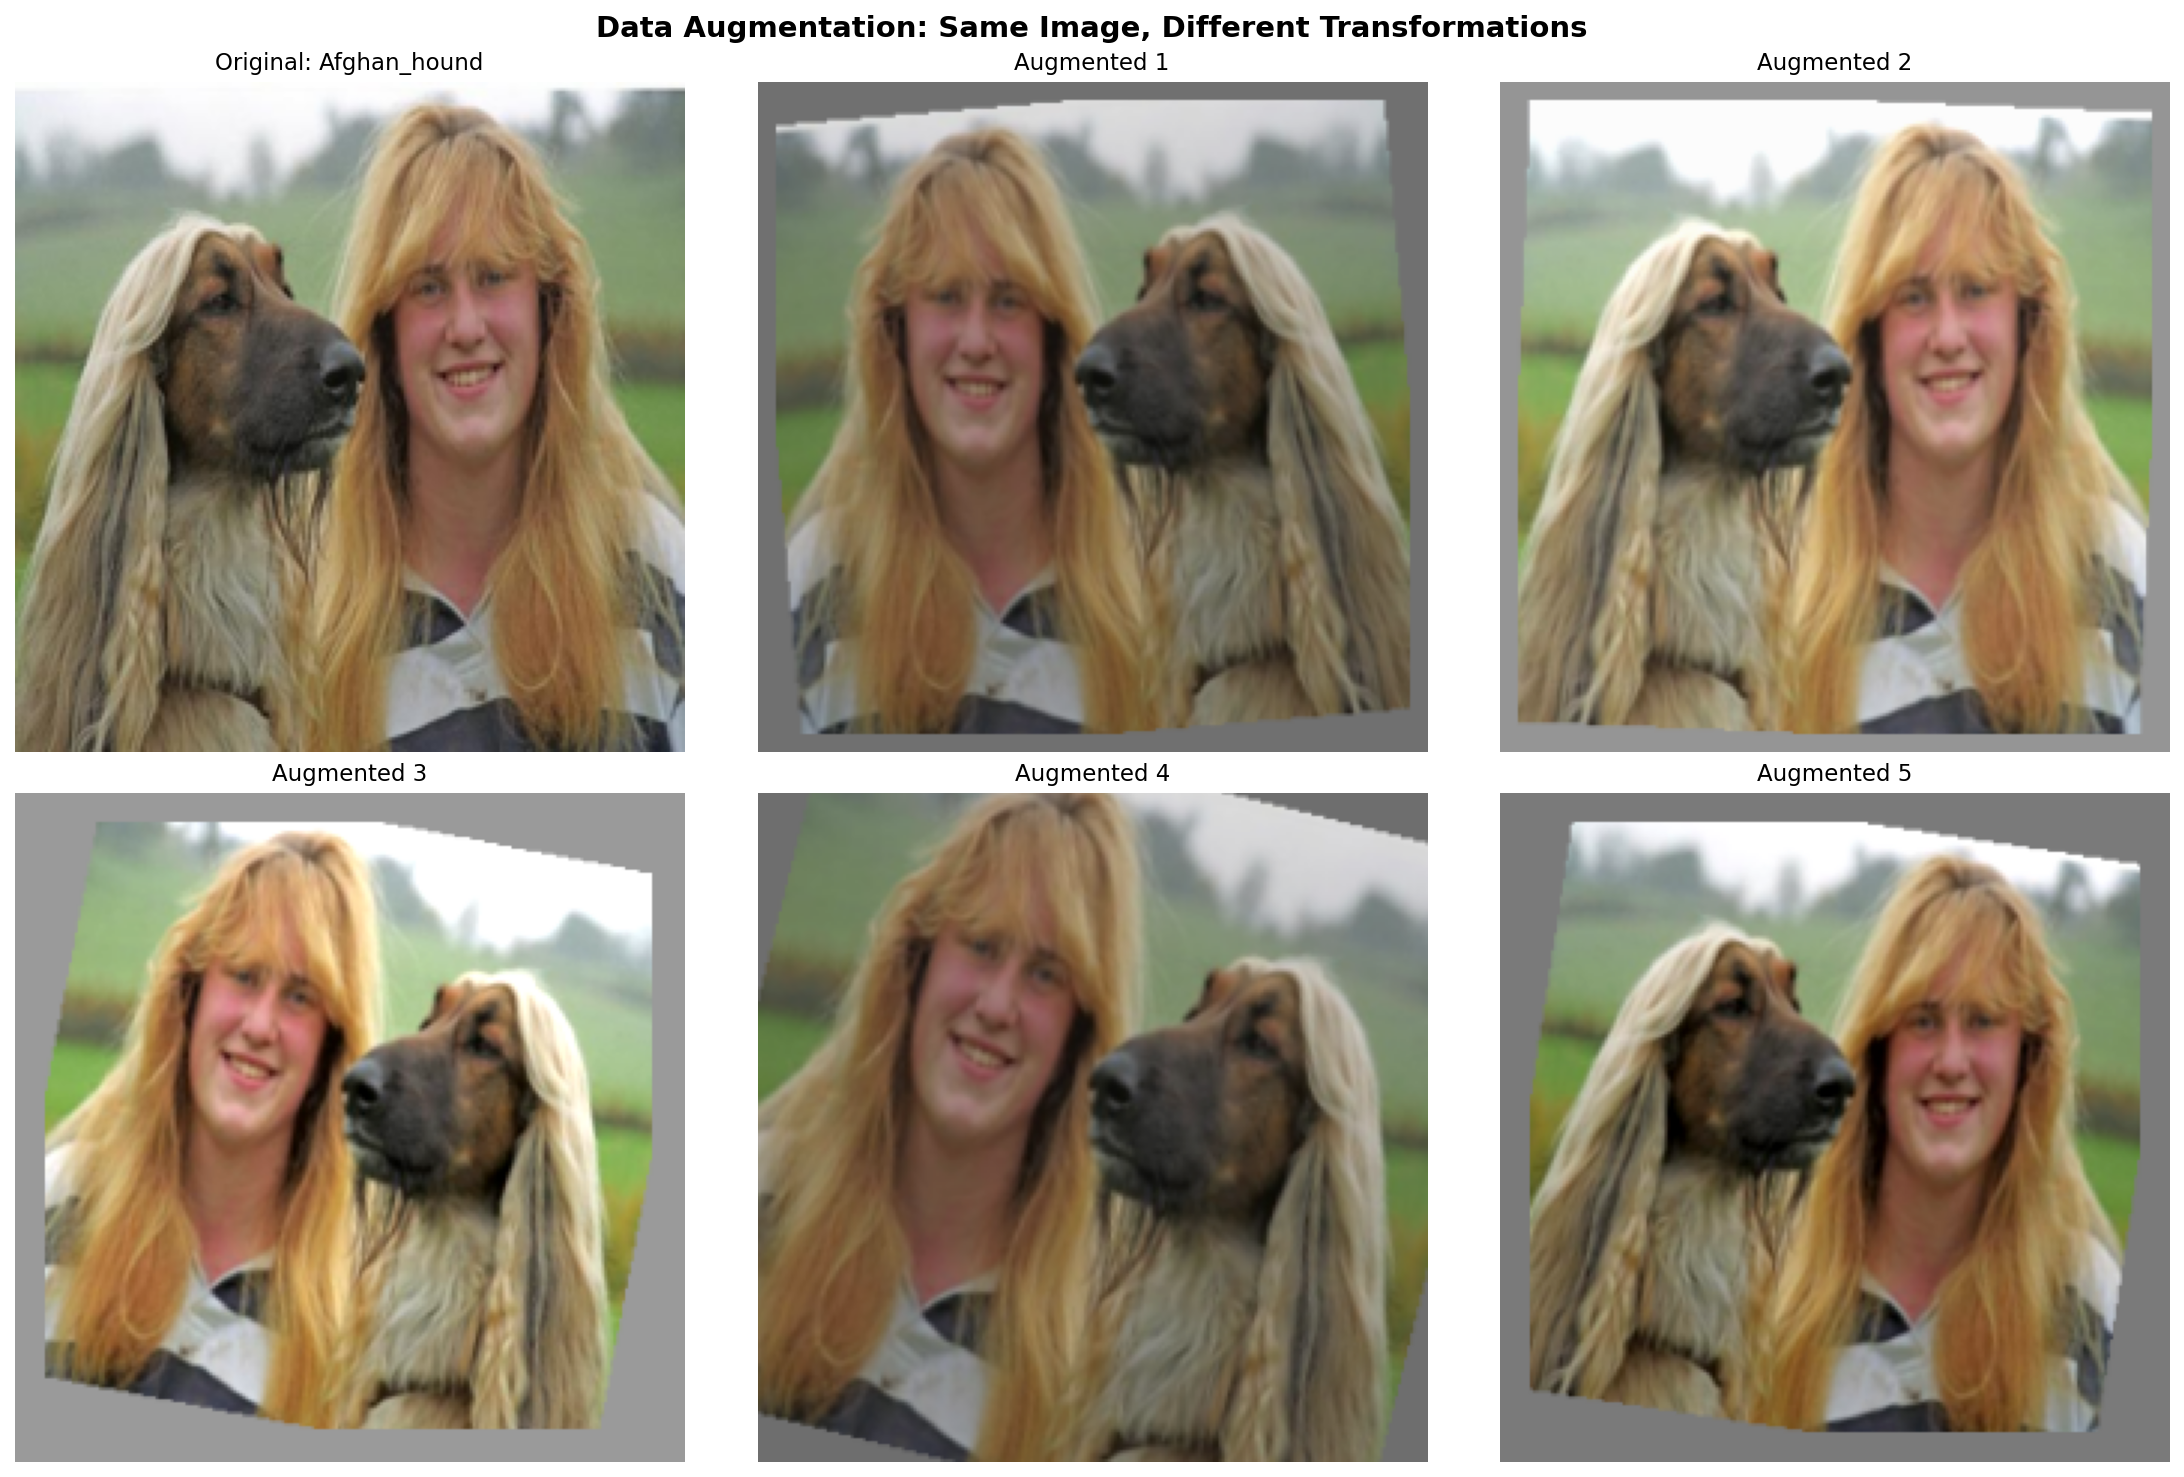
\includegraphics[keepaspectratio]{main_files/figure-pdf/cell-6-output-2.png}}

\begin{verbatim}

✓ Augmentation visualization saved and displayed!
Augmentations: rotation (±15°), flip (50%), zoom (90-110%), brightness/contrast (±20%)
\end{verbatim}

\section{Exploratory Data Analysis}\label{exploratory-data-analysis}

In this section, we explore the dataset characteristics to understand:

\begin{enumerate}
\def\labelenumi{\arabic{enumi}.}
\tightlist
\item
  \textbf{Sample images}: Visual inspection of different breeds
\item
  \textbf{Class distribution}: How balanced are the 120 breed classes?
\item
  \textbf{Image dimensions}: Variation in image sizes and aspect ratios
\item
  \textbf{Data quality}: Any patterns or issues to address before
  training
\end{enumerate}

\begin{Shaded}
\begin{Highlighting}[]
\CommentTok{\# Visualize sample images from different breeds}
\KeywordTok{def}\NormalTok{ show\_sample\_images(train\_df, n\_breeds}\OperatorTok{=}\DecValTok{4}\NormalTok{, images\_per\_breed}\OperatorTok{=}\DecValTok{3}\NormalTok{):}
    \CommentTok{"""Display sample images from random breeds"""}
    
    \CommentTok{\# Sample random breeds}
\NormalTok{    breeds }\OperatorTok{=}\NormalTok{ train\_df[}\StringTok{\textquotesingle{}breed\_name\textquotesingle{}}\NormalTok{].unique()}
\NormalTok{    sample\_breeds }\OperatorTok{=}\NormalTok{ np.random.choice(breeds, size}\OperatorTok{=}\BuiltInTok{min}\NormalTok{(n\_breeds, }\BuiltInTok{len}\NormalTok{(breeds)), replace}\OperatorTok{=}\VariableTok{False}\NormalTok{)}
    
\NormalTok{    fig, axes }\OperatorTok{=}\NormalTok{ plt.subplots(n\_breeds, images\_per\_breed, figsize}\OperatorTok{=}\NormalTok{(}\DecValTok{12}\NormalTok{, n\_breeds}\OperatorTok{*}\DecValTok{3}\NormalTok{))}
    
    \ControlFlowTok{for}\NormalTok{ i, breed }\KeywordTok{in} \BuiltInTok{enumerate}\NormalTok{(sample\_breeds):}
\NormalTok{        breed\_images }\OperatorTok{=}\NormalTok{ train\_df[train\_df[}\StringTok{\textquotesingle{}breed\_name\textquotesingle{}}\NormalTok{] }\OperatorTok{==}\NormalTok{ breed].sample(n}\OperatorTok{=}\NormalTok{images\_per\_breed)}
        
        \ControlFlowTok{for}\NormalTok{ j, (\_, row) }\KeywordTok{in} \BuiltInTok{enumerate}\NormalTok{(breed\_images.iterrows()):}
            \CommentTok{\# Use absolute\_path which has full path from project root}
\NormalTok{            img\_path }\OperatorTok{=}\NormalTok{ Path(}\StringTok{".."}\NormalTok{) }\OperatorTok{/} \StringTok{"data"} \OperatorTok{/} \StringTok{"raw"} \OperatorTok{/}\NormalTok{ row[}\StringTok{\textquotesingle{}file\_path\textquotesingle{}}\NormalTok{]}
\NormalTok{            img }\OperatorTok{=}\NormalTok{ Image.}\BuiltInTok{open}\NormalTok{(img\_path)}
            
\NormalTok{            ax }\OperatorTok{=}\NormalTok{ axes[i, j] }\ControlFlowTok{if}\NormalTok{ n\_breeds }\OperatorTok{\textgreater{}} \DecValTok{1} \ControlFlowTok{else}\NormalTok{ axes[j]}
\NormalTok{            ax.imshow(img)}
\NormalTok{            ax.axis(}\StringTok{\textquotesingle{}off\textquotesingle{}}\NormalTok{)}
            
            \ControlFlowTok{if}\NormalTok{ j }\OperatorTok{==} \DecValTok{0}\NormalTok{:}
\NormalTok{                ax.set\_title(}\SpecialStringTok{f"}\SpecialCharTok{\{}\NormalTok{breed}\SpecialCharTok{\}}\CharTok{\textbackslash{}n}\SpecialCharTok{\{}\NormalTok{img}\SpecialCharTok{.}\NormalTok{size[}\DecValTok{0}\NormalTok{]}\SpecialCharTok{\}}\SpecialStringTok{×}\SpecialCharTok{\{}\NormalTok{img}\SpecialCharTok{.}\NormalTok{size[}\DecValTok{1}\NormalTok{]}\SpecialCharTok{\}}\SpecialStringTok{"}\NormalTok{, fontsize}\OperatorTok{=}\DecValTok{10}\NormalTok{)}
            \ControlFlowTok{else}\NormalTok{:}
\NormalTok{                ax.set\_title(}\SpecialStringTok{f"}\SpecialCharTok{\{}\NormalTok{img}\SpecialCharTok{.}\NormalTok{size[}\DecValTok{0}\NormalTok{]}\SpecialCharTok{\}}\SpecialStringTok{×}\SpecialCharTok{\{}\NormalTok{img}\SpecialCharTok{.}\NormalTok{size[}\DecValTok{1}\NormalTok{]}\SpecialCharTok{\}}\SpecialStringTok{"}\NormalTok{, fontsize}\OperatorTok{=}\DecValTok{9}\NormalTok{)}
    
\NormalTok{    plt.tight\_layout()}
\NormalTok{    plt.savefig(}\StringTok{"../artifacts/figures/sample\_images.png"}\NormalTok{, dpi}\OperatorTok{=}\DecValTok{150}\NormalTok{, bbox\_inches}\OperatorTok{=}\StringTok{\textquotesingle{}tight\textquotesingle{}}\NormalTok{)}

\CommentTok{\# Create figures directory}
\NormalTok{Path(}\StringTok{"../artifacts/figures"}\NormalTok{).mkdir(parents}\OperatorTok{=}\VariableTok{True}\NormalTok{, exist\_ok}\OperatorTok{=}\VariableTok{True}\NormalTok{)}

\CommentTok{\# Show samples}
\NormalTok{np.random.seed(}\DecValTok{42}\NormalTok{)}
\NormalTok{show\_sample\_images(train\_df, n\_breeds}\OperatorTok{=}\DecValTok{4}\NormalTok{, images\_per\_breed}\OperatorTok{=}\DecValTok{3}\NormalTok{)}

\BuiltInTok{print}\NormalTok{(}\StringTok{"}\CharTok{\textbackslash{}n}\StringTok{Sample images showing variety in:"}\NormalTok{)}
\BuiltInTok{print}\NormalTok{(}\StringTok{"  {-} Breed appearance (different sizes, coat colors, facial features)"}\NormalTok{)}
\BuiltInTok{print}\NormalTok{(}\StringTok{"  {-} Image dimensions (various aspect ratios and resolutions)"}\NormalTok{)}
\BuiltInTok{print}\NormalTok{(}\StringTok{"  {-} Photography conditions (backgrounds, lighting, angles)"}\NormalTok{)}
\end{Highlighting}
\end{Shaded}

\begin{verbatim}

Sample images showing variety in:
  - Breed appearance (different sizes, coat colors, facial features)
  - Image dimensions (various aspect ratios and resolutions)
  - Photography conditions (backgrounds, lighting, angles)
\end{verbatim}

\subsection{Image Dimension Analysis}\label{image-dimension-analysis}

Understanding image sizes helps us choose appropriate preprocessing
strategies

\begin{Shaded}
\begin{Highlighting}[]
\CommentTok{\# Analyze image dimensions}
\NormalTok{fig, axes }\OperatorTok{=}\NormalTok{ plt.subplots(}\DecValTok{2}\NormalTok{, }\DecValTok{2}\NormalTok{, figsize}\OperatorTok{=}\NormalTok{(}\DecValTok{14}\NormalTok{, }\DecValTok{10}\NormalTok{))}

\CommentTok{\# Width distribution}
\NormalTok{axes[}\DecValTok{0}\NormalTok{, }\DecValTok{0}\NormalTok{].hist(train\_df[}\StringTok{\textquotesingle{}width\textquotesingle{}}\NormalTok{], bins}\OperatorTok{=}\DecValTok{50}\NormalTok{, edgecolor}\OperatorTok{=}\StringTok{\textquotesingle{}black\textquotesingle{}}\NormalTok{, alpha}\OperatorTok{=}\FloatTok{0.7}\NormalTok{)}
\NormalTok{axes[}\DecValTok{0}\NormalTok{, }\DecValTok{0}\NormalTok{].axvline(train\_df[}\StringTok{\textquotesingle{}width\textquotesingle{}}\NormalTok{].mean(), color}\OperatorTok{=}\StringTok{\textquotesingle{}red\textquotesingle{}}\NormalTok{, linestyle}\OperatorTok{=}\StringTok{\textquotesingle{}{-}{-}\textquotesingle{}}\NormalTok{, }
\NormalTok{                   label}\OperatorTok{=}\SpecialStringTok{f\textquotesingle{}Mean: }\SpecialCharTok{\{}\NormalTok{train\_df[}\StringTok{"width"}\NormalTok{]}\SpecialCharTok{.}\NormalTok{mean()}\SpecialCharTok{:.0f\}}\SpecialStringTok{\textquotesingle{}}\NormalTok{)}
\NormalTok{axes[}\DecValTok{0}\NormalTok{, }\DecValTok{0}\NormalTok{].set\_xlabel(}\StringTok{\textquotesingle{}Width (pixels)\textquotesingle{}}\NormalTok{)}
\NormalTok{axes[}\DecValTok{0}\NormalTok{, }\DecValTok{0}\NormalTok{].set\_ylabel(}\StringTok{\textquotesingle{}Frequency\textquotesingle{}}\NormalTok{)}
\NormalTok{axes[}\DecValTok{0}\NormalTok{, }\DecValTok{0}\NormalTok{].set\_title(}\StringTok{\textquotesingle{}Image Width Distribution\textquotesingle{}}\NormalTok{)}
\NormalTok{axes[}\DecValTok{0}\NormalTok{, }\DecValTok{0}\NormalTok{].legend()}
\NormalTok{axes[}\DecValTok{0}\NormalTok{, }\DecValTok{0}\NormalTok{].grid(alpha}\OperatorTok{=}\FloatTok{0.3}\NormalTok{)}

\CommentTok{\# Height distribution}
\NormalTok{axes[}\DecValTok{0}\NormalTok{, }\DecValTok{1}\NormalTok{].hist(train\_df[}\StringTok{\textquotesingle{}height\textquotesingle{}}\NormalTok{], bins}\OperatorTok{=}\DecValTok{50}\NormalTok{, edgecolor}\OperatorTok{=}\StringTok{\textquotesingle{}black\textquotesingle{}}\NormalTok{, alpha}\OperatorTok{=}\FloatTok{0.7}\NormalTok{)}
\NormalTok{axes[}\DecValTok{0}\NormalTok{, }\DecValTok{1}\NormalTok{].axvline(train\_df[}\StringTok{\textquotesingle{}height\textquotesingle{}}\NormalTok{].mean(), color}\OperatorTok{=}\StringTok{\textquotesingle{}red\textquotesingle{}}\NormalTok{, linestyle}\OperatorTok{=}\StringTok{\textquotesingle{}{-}{-}\textquotesingle{}}\NormalTok{,}
\NormalTok{                   label}\OperatorTok{=}\SpecialStringTok{f\textquotesingle{}Mean: }\SpecialCharTok{\{}\NormalTok{train\_df[}\StringTok{"height"}\NormalTok{]}\SpecialCharTok{.}\NormalTok{mean()}\SpecialCharTok{:.0f\}}\SpecialStringTok{\textquotesingle{}}\NormalTok{)}
\NormalTok{axes[}\DecValTok{0}\NormalTok{, }\DecValTok{1}\NormalTok{].set\_xlabel(}\StringTok{\textquotesingle{}Height (pixels)\textquotesingle{}}\NormalTok{)}
\NormalTok{axes[}\DecValTok{0}\NormalTok{, }\DecValTok{1}\NormalTok{].set\_ylabel(}\StringTok{\textquotesingle{}Frequency\textquotesingle{}}\NormalTok{)}
\NormalTok{axes[}\DecValTok{0}\NormalTok{, }\DecValTok{1}\NormalTok{].set\_title(}\StringTok{\textquotesingle{}Image Height Distribution\textquotesingle{}}\NormalTok{)}
\NormalTok{axes[}\DecValTok{0}\NormalTok{, }\DecValTok{1}\NormalTok{].legend()}
\NormalTok{axes[}\DecValTok{0}\NormalTok{, }\DecValTok{1}\NormalTok{].grid(alpha}\OperatorTok{=}\FloatTok{0.3}\NormalTok{)}

\CommentTok{\# Aspect ratio}
\NormalTok{train\_df[}\StringTok{\textquotesingle{}aspect\_ratio\textquotesingle{}}\NormalTok{] }\OperatorTok{=}\NormalTok{ train\_df[}\StringTok{\textquotesingle{}width\textquotesingle{}}\NormalTok{] }\OperatorTok{/}\NormalTok{ train\_df[}\StringTok{\textquotesingle{}height\textquotesingle{}}\NormalTok{]}
\NormalTok{axes[}\DecValTok{1}\NormalTok{, }\DecValTok{0}\NormalTok{].hist(train\_df[}\StringTok{\textquotesingle{}aspect\_ratio\textquotesingle{}}\NormalTok{], bins}\OperatorTok{=}\DecValTok{50}\NormalTok{, edgecolor}\OperatorTok{=}\StringTok{\textquotesingle{}black\textquotesingle{}}\NormalTok{, alpha}\OperatorTok{=}\FloatTok{0.7}\NormalTok{)}
\NormalTok{axes[}\DecValTok{1}\NormalTok{, }\DecValTok{0}\NormalTok{].axvline(}\FloatTok{1.0}\NormalTok{, color}\OperatorTok{=}\StringTok{\textquotesingle{}green\textquotesingle{}}\NormalTok{, linestyle}\OperatorTok{=}\StringTok{\textquotesingle{}{-}{-}\textquotesingle{}}\NormalTok{, label}\OperatorTok{=}\StringTok{\textquotesingle{}Square (1:1)\textquotesingle{}}\NormalTok{)}
\NormalTok{axes[}\DecValTok{1}\NormalTok{, }\DecValTok{0}\NormalTok{].set\_xlabel(}\StringTok{\textquotesingle{}Aspect Ratio (width/height)\textquotesingle{}}\NormalTok{)}
\NormalTok{axes[}\DecValTok{1}\NormalTok{, }\DecValTok{0}\NormalTok{].set\_ylabel(}\StringTok{\textquotesingle{}Frequency\textquotesingle{}}\NormalTok{)}
\NormalTok{axes[}\DecValTok{1}\NormalTok{, }\DecValTok{0}\NormalTok{].set\_title(}\StringTok{\textquotesingle{}Aspect Ratio Distribution\textquotesingle{}}\NormalTok{)}
\NormalTok{axes[}\DecValTok{1}\NormalTok{, }\DecValTok{0}\NormalTok{].legend()}
\NormalTok{axes[}\DecValTok{1}\NormalTok{, }\DecValTok{0}\NormalTok{].grid(alpha}\OperatorTok{=}\FloatTok{0.3}\NormalTok{)}
\end{Highlighting}
\end{Shaded}

\begin{Shaded}
\begin{Highlighting}[]
\CommentTok{\# Scatter: width vs height}
\NormalTok{axes[}\DecValTok{1}\NormalTok{, }\DecValTok{1}\NormalTok{].scatter(train\_df[}\StringTok{\textquotesingle{}width\textquotesingle{}}\NormalTok{], train\_df[}\StringTok{\textquotesingle{}height\textquotesingle{}}\NormalTok{], alpha}\OperatorTok{=}\FloatTok{0.3}\NormalTok{, s}\OperatorTok{=}\DecValTok{1}\NormalTok{)}
\NormalTok{axes[}\DecValTok{1}\NormalTok{, }\DecValTok{1}\NormalTok{].plot([}\DecValTok{0}\NormalTok{, }\DecValTok{1000}\NormalTok{], [}\DecValTok{0}\NormalTok{, }\DecValTok{1000}\NormalTok{], }\StringTok{\textquotesingle{}r{-}{-}\textquotesingle{}}\NormalTok{, label}\OperatorTok{=}\StringTok{\textquotesingle{}Square\textquotesingle{}}\NormalTok{, linewidth}\OperatorTok{=}\DecValTok{1}\NormalTok{)}
\NormalTok{axes[}\DecValTok{1}\NormalTok{, }\DecValTok{1}\NormalTok{].set\_xlabel(}\StringTok{\textquotesingle{}Width (pixels)\textquotesingle{}}\NormalTok{)}
\NormalTok{axes[}\DecValTok{1}\NormalTok{, }\DecValTok{1}\NormalTok{].set\_ylabel(}\StringTok{\textquotesingle{}Height (pixels)\textquotesingle{}}\NormalTok{)}
\NormalTok{axes[}\DecValTok{1}\NormalTok{, }\DecValTok{1}\NormalTok{].set\_title(}\StringTok{\textquotesingle{}Width vs Height Scatter\textquotesingle{}}\NormalTok{)}
\NormalTok{axes[}\DecValTok{1}\NormalTok{, }\DecValTok{1}\NormalTok{].legend()}
\NormalTok{axes[}\DecValTok{1}\NormalTok{, }\DecValTok{1}\NormalTok{].grid(alpha}\OperatorTok{=}\FloatTok{0.3}\NormalTok{)}
\NormalTok{axes[}\DecValTok{1}\NormalTok{, }\DecValTok{1}\NormalTok{].set\_xlim(}\DecValTok{0}\NormalTok{, train\_df[}\StringTok{\textquotesingle{}width\textquotesingle{}}\NormalTok{].}\BuiltInTok{max}\NormalTok{() }\OperatorTok{+} \DecValTok{50}\NormalTok{)}
\NormalTok{axes[}\DecValTok{1}\NormalTok{, }\DecValTok{1}\NormalTok{].set\_ylim(}\DecValTok{0}\NormalTok{, train\_df[}\StringTok{\textquotesingle{}height\textquotesingle{}}\NormalTok{].}\BuiltInTok{max}\NormalTok{() }\OperatorTok{+} \DecValTok{50}\NormalTok{)}

\NormalTok{plt.tight\_layout()}
\NormalTok{plt.savefig(}\StringTok{"../artifacts/figures/image\_dimensions.png"}\NormalTok{, dpi}\OperatorTok{=}\DecValTok{150}\NormalTok{, bbox\_inches}\OperatorTok{=}\StringTok{\textquotesingle{}tight\textquotesingle{}}\NormalTok{)}

\BuiltInTok{print}\NormalTok{(}\SpecialStringTok{f"}\CharTok{\textbackslash{}n}\SpecialStringTok{Image Dimension Statistics:"}\NormalTok{)}
\BuiltInTok{print}\NormalTok{(}\SpecialStringTok{f"  Width  {-} Mean: }\SpecialCharTok{\{}\NormalTok{train\_df[}\StringTok{\textquotesingle{}width\textquotesingle{}}\NormalTok{]}\SpecialCharTok{.}\NormalTok{mean()}\SpecialCharTok{:.0f\}}\SpecialStringTok{, Std: }\SpecialCharTok{\{}\NormalTok{train\_df[}\StringTok{\textquotesingle{}width\textquotesingle{}}\NormalTok{]}\SpecialCharTok{.}\NormalTok{std()}\SpecialCharTok{:.0f\}}\SpecialStringTok{, Range: [}\SpecialCharTok{\{}\NormalTok{train\_df[}\StringTok{\textquotesingle{}width\textquotesingle{}}\NormalTok{]}\SpecialCharTok{.}\BuiltInTok{min}\NormalTok{()}\SpecialCharTok{\}}\SpecialStringTok{, }\SpecialCharTok{\{}\NormalTok{train\_df[}\StringTok{\textquotesingle{}width\textquotesingle{}}\NormalTok{]}\SpecialCharTok{.}\BuiltInTok{max}\NormalTok{()}\SpecialCharTok{\}}\SpecialStringTok{]"}\NormalTok{)}
\BuiltInTok{print}\NormalTok{(}\SpecialStringTok{f"  Height {-} Mean: }\SpecialCharTok{\{}\NormalTok{train\_df[}\StringTok{\textquotesingle{}height\textquotesingle{}}\NormalTok{]}\SpecialCharTok{.}\NormalTok{mean()}\SpecialCharTok{:.0f\}}\SpecialStringTok{, Std: }\SpecialCharTok{\{}\NormalTok{train\_df[}\StringTok{\textquotesingle{}height\textquotesingle{}}\NormalTok{]}\SpecialCharTok{.}\NormalTok{std()}\SpecialCharTok{:.0f\}}\SpecialStringTok{, Range: [}\SpecialCharTok{\{}\NormalTok{train\_df[}\StringTok{\textquotesingle{}height\textquotesingle{}}\NormalTok{]}\SpecialCharTok{.}\BuiltInTok{min}\NormalTok{()}\SpecialCharTok{\}}\SpecialStringTok{, }\SpecialCharTok{\{}\NormalTok{train\_df[}\StringTok{\textquotesingle{}height\textquotesingle{}}\NormalTok{]}\SpecialCharTok{.}\BuiltInTok{max}\NormalTok{()}\SpecialCharTok{\}}\SpecialStringTok{]"}\NormalTok{)}
\BuiltInTok{print}\NormalTok{(}\SpecialStringTok{f"  Aspect Ratio {-} Mean: }\SpecialCharTok{\{}\NormalTok{train\_df[}\StringTok{\textquotesingle{}aspect\_ratio\textquotesingle{}}\NormalTok{]}\SpecialCharTok{.}\NormalTok{mean()}\SpecialCharTok{:.2f\}}\SpecialStringTok{, Std: }\SpecialCharTok{\{}\NormalTok{train\_df[}\StringTok{\textquotesingle{}aspect\_ratio\textquotesingle{}}\NormalTok{]}\SpecialCharTok{.}\NormalTok{std()}\SpecialCharTok{:.2f\}}\SpecialStringTok{"}\NormalTok{)}
\BuiltInTok{print}\NormalTok{(}\SpecialStringTok{f"}\CharTok{\textbackslash{}n}\SpecialStringTok{Resizing strategy: All images will be resized to 224×224 for CNN input (standard for ImageNet pre{-}trained models)"}\NormalTok{)}
\end{Highlighting}
\end{Shaded}

\begin{verbatim}

Image Dimension Statistics:
  Width  - Mean: 443, Std: 145, Range: [100, 3264]
  Height - Mean: 386, Std: 127, Range: [100, 2562]
  Aspect Ratio - Mean: 1.19, Std: 0.30

Resizing strategy: All images will be resized to 224×224 for CNN input (standard for ImageNet pre-trained models)
\end{verbatim}

\begin{Shaded}
\begin{Highlighting}[]
\CommentTok{\# Analyze class distribution}
\NormalTok{breed\_counts }\OperatorTok{=}\NormalTok{ train\_df[}\StringTok{\textquotesingle{}breed\_name\textquotesingle{}}\NormalTok{].value\_counts().sort\_values(ascending}\OperatorTok{=}\VariableTok{False}\NormalTok{)}

\NormalTok{fig, axes }\OperatorTok{=}\NormalTok{ plt.subplots(}\DecValTok{1}\NormalTok{, }\DecValTok{2}\NormalTok{, figsize}\OperatorTok{=}\NormalTok{(}\DecValTok{16}\NormalTok{, }\DecValTok{5}\NormalTok{))}

\CommentTok{\# Plot 1: Top 20 breeds}
\NormalTok{axes[}\DecValTok{0}\NormalTok{].barh(breed\_counts.head(}\DecValTok{20}\NormalTok{).index[::}\OperatorTok{{-}}\DecValTok{1}\NormalTok{], breed\_counts.head(}\DecValTok{20}\NormalTok{).values[::}\OperatorTok{{-}}\DecValTok{1}\NormalTok{])}
\NormalTok{axes[}\DecValTok{0}\NormalTok{].set\_xlabel(}\StringTok{\textquotesingle{}Number of Images\textquotesingle{}}\NormalTok{)}
\NormalTok{axes[}\DecValTok{0}\NormalTok{].set\_title(}\StringTok{\textquotesingle{}Top 20 Breeds by Image Count (Training Set)\textquotesingle{}}\NormalTok{)}
\NormalTok{axes[}\DecValTok{0}\NormalTok{].grid(axis}\OperatorTok{=}\StringTok{\textquotesingle{}x\textquotesingle{}}\NormalTok{, alpha}\OperatorTok{=}\FloatTok{0.3}\NormalTok{)}

\CommentTok{\# Plot 2: Distribution histogram}
\NormalTok{axes[}\DecValTok{1}\NormalTok{].hist(breed\_counts.values, bins}\OperatorTok{=}\DecValTok{30}\NormalTok{, edgecolor}\OperatorTok{=}\StringTok{\textquotesingle{}black\textquotesingle{}}\NormalTok{, alpha}\OperatorTok{=}\FloatTok{0.7}\NormalTok{)}
\NormalTok{axes[}\DecValTok{1}\NormalTok{].axvline(breed\_counts.mean(), color}\OperatorTok{=}\StringTok{\textquotesingle{}red\textquotesingle{}}\NormalTok{, linestyle}\OperatorTok{=}\StringTok{\textquotesingle{}{-}{-}\textquotesingle{}}\NormalTok{, label}\OperatorTok{=}\SpecialStringTok{f\textquotesingle{}Mean: }\SpecialCharTok{\{}\NormalTok{breed\_counts}\SpecialCharTok{.}\NormalTok{mean()}\SpecialCharTok{:.1f\}}\SpecialStringTok{\textquotesingle{}}\NormalTok{)}
\NormalTok{axes[}\DecValTok{1}\NormalTok{].axvline(breed\_counts.median(), color}\OperatorTok{=}\StringTok{\textquotesingle{}green\textquotesingle{}}\NormalTok{, linestyle}\OperatorTok{=}\StringTok{\textquotesingle{}{-}{-}\textquotesingle{}}\NormalTok{, label}\OperatorTok{=}\SpecialStringTok{f\textquotesingle{}Median: }\SpecialCharTok{\{}\NormalTok{breed\_counts}\SpecialCharTok{.}\NormalTok{median()}\SpecialCharTok{:.1f\}}\SpecialStringTok{\textquotesingle{}}\NormalTok{)}
\NormalTok{axes[}\DecValTok{1}\NormalTok{].set\_xlabel(}\StringTok{\textquotesingle{}Number of Images per Breed\textquotesingle{}}\NormalTok{)}
\NormalTok{axes[}\DecValTok{1}\NormalTok{].set\_ylabel(}\StringTok{\textquotesingle{}Number of Breeds\textquotesingle{}}\NormalTok{)}
\NormalTok{axes[}\DecValTok{1}\NormalTok{].set\_title(}\StringTok{\textquotesingle{}Distribution of Images Across Breeds\textquotesingle{}}\NormalTok{)}
\NormalTok{axes[}\DecValTok{1}\NormalTok{].legend()}
\NormalTok{axes[}\DecValTok{1}\NormalTok{].grid(alpha}\OperatorTok{=}\FloatTok{0.3}\NormalTok{)}

\NormalTok{plt.tight\_layout()}
\NormalTok{plt.savefig(}\StringTok{"../artifacts/figures/breed\_distribution.png"}\NormalTok{, dpi}\OperatorTok{=}\DecValTok{150}\NormalTok{, bbox\_inches}\OperatorTok{=}\StringTok{\textquotesingle{}tight\textquotesingle{}}\NormalTok{)}

\BuiltInTok{print}\NormalTok{(}\SpecialStringTok{f"}\CharTok{\textbackslash{}n}\SpecialStringTok{Class Balance Analysis:"}\NormalTok{)}
\BuiltInTok{print}\NormalTok{(}\SpecialStringTok{f"  Total breeds: }\SpecialCharTok{\{}\BuiltInTok{len}\NormalTok{(breed\_counts)}\SpecialCharTok{\}}\SpecialStringTok{"}\NormalTok{)}
\BuiltInTok{print}\NormalTok{(}\SpecialStringTok{f"  Min images per breed: }\SpecialCharTok{\{}\NormalTok{breed\_counts}\SpecialCharTok{.}\BuiltInTok{min}\NormalTok{()}\SpecialCharTok{\}}\SpecialStringTok{"}\NormalTok{)}
\BuiltInTok{print}\NormalTok{(}\SpecialStringTok{f"  Max images per breed: }\SpecialCharTok{\{}\NormalTok{breed\_counts}\SpecialCharTok{.}\BuiltInTok{max}\NormalTok{()}\SpecialCharTok{\}}\SpecialStringTok{"}\NormalTok{)}
\BuiltInTok{print}\NormalTok{(}\SpecialStringTok{f"  Mean images per breed: }\SpecialCharTok{\{}\NormalTok{breed\_counts}\SpecialCharTok{.}\NormalTok{mean()}\SpecialCharTok{:.1f\}}\SpecialStringTok{"}\NormalTok{)}
\BuiltInTok{print}\NormalTok{(}\SpecialStringTok{f"  Std images per breed: }\SpecialCharTok{\{}\NormalTok{breed\_counts}\SpecialCharTok{.}\NormalTok{std()}\SpecialCharTok{:.1f\}}\SpecialStringTok{"}\NormalTok{)}
\BuiltInTok{print}\NormalTok{(}\SpecialStringTok{f"  Imbalance ratio (max/min): }\SpecialCharTok{\{}\NormalTok{breed\_counts}\SpecialCharTok{.}\BuiltInTok{max}\NormalTok{()}\OperatorTok{/}\NormalTok{breed\_counts}\SpecialCharTok{.}\BuiltInTok{min}\NormalTok{()}\SpecialCharTok{:.2f\}}\SpecialStringTok{x"}\NormalTok{)}

\BuiltInTok{print}\NormalTok{(}\SpecialStringTok{f"}\CharTok{\textbackslash{}n}\SpecialStringTok{Most common breeds:"}\NormalTok{)}
\ControlFlowTok{for}\NormalTok{ breed, count }\KeywordTok{in}\NormalTok{ breed\_counts.head(}\DecValTok{5}\NormalTok{).items():}
    \BuiltInTok{print}\NormalTok{(}\SpecialStringTok{f"  }\SpecialCharTok{\{}\NormalTok{breed}\SpecialCharTok{\}}\SpecialStringTok{: }\SpecialCharTok{\{}\NormalTok{count}\SpecialCharTok{\}}\SpecialStringTok{ images"}\NormalTok{)}
    
\BuiltInTok{print}\NormalTok{(}\SpecialStringTok{f"}\CharTok{\textbackslash{}n}\SpecialStringTok{Least common breeds:"}\NormalTok{)}
\ControlFlowTok{for}\NormalTok{ breed, count }\KeywordTok{in}\NormalTok{ breed\_counts.tail(}\DecValTok{5}\NormalTok{).items():}
    \BuiltInTok{print}\NormalTok{(}\SpecialStringTok{f"  }\SpecialCharTok{\{}\NormalTok{breed}\SpecialCharTok{\}}\SpecialStringTok{: }\SpecialCharTok{\{}\NormalTok{count}\SpecialCharTok{\}}\SpecialStringTok{ images"}\NormalTok{)}
\end{Highlighting}
\end{Shaded}

\begin{verbatim}

Class Balance Analysis:
  Total breeds: 120
  Min images per breed: 119
  Max images per breed: 202
  Mean images per breed: 137.6
  Std images per breed: 18.6
  Imbalance ratio (max/min): 1.70x

Most common breeds:
  Maltese_dog: 202 images
  Afghan_hound: 192 images
  Scottish_deerhound: 186 images
  Pomeranian: 176 images
  Samoyed: 175 images

Least common breeds:
  clumber: 120 images
  Border_collie: 120 images
  Pekinese: 120 images
  Bouvier_des_Flandres: 120 images
  redbone: 119 images
\end{verbatim}

\begin{Shaded}
\begin{Highlighting}[]
\NormalTok{fig, ax }\OperatorTok{=}\NormalTok{ plt.subplots(}\DecValTok{1}\NormalTok{, }\DecValTok{1}\NormalTok{, figsize}\OperatorTok{=}\NormalTok{(}\DecValTok{12}\NormalTok{, }\DecValTok{6}\NormalTok{))}

\NormalTok{breed\_counts\_sorted }\OperatorTok{=}\NormalTok{ breed\_counts.sort\_values(ascending}\OperatorTok{=}\VariableTok{True}\NormalTok{)}
\NormalTok{colors }\OperatorTok{=}\NormalTok{ [}\StringTok{\textquotesingle{}red\textquotesingle{}} \ControlFlowTok{if}\NormalTok{ x }\OperatorTok{\textless{}} \DecValTok{130} \ControlFlowTok{else} \StringTok{\textquotesingle{}orange\textquotesingle{}} \ControlFlowTok{if}\NormalTok{ x }\OperatorTok{\textless{}} \DecValTok{150} \ControlFlowTok{else} \StringTok{\textquotesingle{}green\textquotesingle{}} 
          \ControlFlowTok{for}\NormalTok{ x }\KeywordTok{in}\NormalTok{ breed\_counts\_sorted.values]}

\NormalTok{ax.barh(}\BuiltInTok{range}\NormalTok{(}\BuiltInTok{len}\NormalTok{(breed\_counts\_sorted)), breed\_counts\_sorted.values, color}\OperatorTok{=}\NormalTok{colors)}
\NormalTok{ax.axvline(}\FloatTok{137.6}\NormalTok{, color}\OperatorTok{=}\StringTok{\textquotesingle{}blue\textquotesingle{}}\NormalTok{, linestyle}\OperatorTok{=}\StringTok{\textquotesingle{}{-}{-}\textquotesingle{}}\NormalTok{, linewidth}\OperatorTok{=}\DecValTok{2}\NormalTok{, label}\OperatorTok{=}\StringTok{\textquotesingle{}Mean (138)\textquotesingle{}}\NormalTok{)}
\NormalTok{ax.axvline(}\DecValTok{150}\NormalTok{, color}\OperatorTok{=}\StringTok{\textquotesingle{}orange\textquotesingle{}}\NormalTok{, linestyle}\OperatorTok{=}\StringTok{\textquotesingle{}{-}{-}\textquotesingle{}}\NormalTok{, linewidth}\OperatorTok{=}\DecValTok{1}\NormalTok{, alpha}\OperatorTok{=}\FloatTok{0.7}\NormalTok{, label}\OperatorTok{=}\StringTok{\textquotesingle{}Adequate (150)\textquotesingle{}}\NormalTok{)}

\NormalTok{ax.set\_xlabel(}\StringTok{\textquotesingle{}Number of Training Images\textquotesingle{}}\NormalTok{)}
\NormalTok{ax.set\_ylabel(}\StringTok{\textquotesingle{}Breed Index\textquotesingle{}}\NormalTok{)}
\NormalTok{ax.set\_title(}\StringTok{\textquotesingle{}Training Sample Size per Breed (Sorted)}\CharTok{\textbackslash{}n}\StringTok{Red: \textless{}130 samples, Orange: 130{-}150, Green: \textgreater{}150\textquotesingle{}}\NormalTok{)}
\NormalTok{ax.legend()}
\NormalTok{ax.grid(axis}\OperatorTok{=}\StringTok{\textquotesingle{}x\textquotesingle{}}\NormalTok{, alpha}\OperatorTok{=}\FloatTok{0.3}\NormalTok{)}

\CommentTok{\# Add text annotation}
\NormalTok{ax.text(}\FloatTok{0.02}\NormalTok{, }\FloatTok{0.98}\NormalTok{, }\SpecialStringTok{f\textquotesingle{}}\SpecialCharTok{\{}\NormalTok{(breed\_counts }\OperatorTok{\textless{}} \DecValTok{130}\NormalTok{)}\SpecialCharTok{.}\BuiltInTok{sum}\NormalTok{()}\SpecialCharTok{\}}\SpecialStringTok{ breeds with \textless{}130 samples\textquotesingle{}}\NormalTok{, }
\NormalTok{        transform}\OperatorTok{=}\NormalTok{ax.transAxes, va}\OperatorTok{=}\StringTok{\textquotesingle{}top\textquotesingle{}}\NormalTok{, bbox}\OperatorTok{=}\BuiltInTok{dict}\NormalTok{(boxstyle}\OperatorTok{=}\StringTok{\textquotesingle{}round\textquotesingle{}}\NormalTok{, facecolor}\OperatorTok{=}\StringTok{\textquotesingle{}wheat\textquotesingle{}}\NormalTok{))}

\NormalTok{plt.tight\_layout()}
\NormalTok{plt.savefig(}\StringTok{"../artifacts/figures/sample\_adequacy.png"}\NormalTok{, dpi}\OperatorTok{=}\DecValTok{150}\NormalTok{, bbox\_inches}\OperatorTok{=}\StringTok{\textquotesingle{}tight\textquotesingle{}}\NormalTok{)}

\BuiltInTok{print}\NormalTok{(}\SpecialStringTok{f"}\CharTok{\textbackslash{}n}\SpecialStringTok{Sample Adequacy Summary:"}\NormalTok{)}
\BuiltInTok{print}\NormalTok{(}\SpecialStringTok{f"  Breeds with \textless{}130 samples (may underperform): }\SpecialCharTok{\{}\NormalTok{(breed\_counts }\OperatorTok{\textless{}} \DecValTok{130}\NormalTok{)}\SpecialCharTok{.}\BuiltInTok{sum}\NormalTok{()}\SpecialCharTok{\}}\SpecialStringTok{"}\NormalTok{)}
\BuiltInTok{print}\NormalTok{(}\SpecialStringTok{f"  Breeds with 130{-}150 samples (adequate): }\SpecialCharTok{\{}\NormalTok{((breed\_counts }\OperatorTok{\textgreater{}=} \DecValTok{130}\NormalTok{) }\OperatorTok{\&}\NormalTok{ (breed\_counts }\OperatorTok{\textless{}} \DecValTok{150}\NormalTok{))}\SpecialCharTok{.}\BuiltInTok{sum}\NormalTok{()}\SpecialCharTok{\}}\SpecialStringTok{"}\NormalTok{)}
\BuiltInTok{print}\NormalTok{(}\SpecialStringTok{f"  Breeds with \textgreater{}150 samples (good): }\SpecialCharTok{\{}\NormalTok{(breed\_counts }\OperatorTok{\textgreater{}=} \DecValTok{150}\NormalTok{)}\SpecialCharTok{.}\BuiltInTok{sum}\NormalTok{()}\SpecialCharTok{\}}\SpecialStringTok{"}\NormalTok{)}
\BuiltInTok{print}\NormalTok{(}\SpecialStringTok{f"}\CharTok{\textbackslash{}n}\SpecialStringTok{Conclusion: }\SpecialCharTok{\{}\NormalTok{(breed\_counts }\OperatorTok{\textless{}} \DecValTok{130}\NormalTok{)}\SpecialCharTok{.}\BuiltInTok{sum}\NormalTok{()}\SpecialCharTok{\}}\SpecialStringTok{ breeds may show lower accuracy due to limited training data."}\NormalTok{)}
\end{Highlighting}
\end{Shaded}

\begin{verbatim}

Sample Adequacy Summary:
  Breeds with <130 samples (may underperform): 62
  Breeds with 130-150 samples (adequate): 28
  Breeds with >150 samples (good): 30

Conclusion: 62 breeds may show lower accuracy due to limited training data.
\end{verbatim}

\section{Models}\label{models}

\begin{itemize}
\tightlist
\item
  Baselines: Start with simple baselines (mean/last value,
  logistic/linear).
\item
  Candidates: Consider tree-based (RF/XGBoost), linear, neural, or
  specialized models.
\item
  Hyperparameters: Document search space and defaults.
\end{itemize}

\begin{center}\rule{0.5\linewidth}{0.5pt}\end{center}

\begin{itemize}
\tightlist
\item
  Experiment Plan: A compact matrix listing planned model families, key
  features, and parameters to try.
\end{itemize}

\section{Training}\label{training}

\begin{itemize}
\tightlist
\item
  Strategy: Train/validation/test split strategy, cross-validation, and
  seeds.
\item
  Reproducibility: Deterministic seeds, config files, and artifact
  logging.
\item
  Compute: Hardware, runtime, and cost notes.
\end{itemize}

\begin{center}\rule{0.5\linewidth}{0.5pt}\end{center}

\begin{itemize}
\tightlist
\item
  Split Strategy \& Leakage: Explicitly state split logic (time-aware vs
  random), test size, and leakage mitigations.
\item
  Reproducibility Checklist: Config use, seeds, artifact locations,
  environment capture (Python + key pkg versions).
\end{itemize}

\begin{Shaded}
\begin{Highlighting}[]
\CommentTok{\# Evaluate model and save simple plots}
\ImportTok{import}\NormalTok{ sys}
\ImportTok{from}\NormalTok{ pathlib }\ImportTok{import}\NormalTok{ Path}
\NormalTok{sys.path.append(}\BuiltInTok{str}\NormalTok{(Path.cwd() }\OperatorTok{/} \StringTok{\textquotesingle{}src\textquotesingle{}}\NormalTok{))}
\ImportTok{from}\NormalTok{ dbc.}\BuiltInTok{eval} \ImportTok{import}\NormalTok{ main }\ImportTok{as}\NormalTok{ eval\_main}
\NormalTok{CONFIG }\OperatorTok{=} \StringTok{\textquotesingle{}configs/exp\_baseline.yaml\textquotesingle{}}
\NormalTok{eval\_main(CONFIG)}
\end{Highlighting}
\end{Shaded}

\begin{Highlighting}
\textcolor{black}{FileNotFoundError: [Errno 2] No such file or directory: 'configs/exp\_baseline.yaml'}
\textcolor{black}{}\textcolor{QuartoInternalColor1}{---------------------------------------------------------------------------}\textcolor{QuartoInternalColor2}{}
\textcolor{QuartoInternalColor2}{}\textcolor{QuartoInternalColor1}{FileNotFoundError}\textcolor{QuartoInternalColor2}{                         Traceback (most recent call last)}
\textcolor{QuartoInternalColor2}{Cell }\textcolor{QuartoInternalColor3}{In[134], line 7}\textcolor{QuartoInternalColor2}{}
\textcolor{QuartoInternalColor2}{}\textcolor{QuartoInternalColor4}{      5}\textcolor{QuartoInternalColor2}{ }\textcolor{QuartoInternalColor5}{from}\textcolor{QuartoInternalColor2}{ }\textcolor{QuartoInternalColor6}{dbc}\textcolor{QuartoInternalColor2}{}\textcolor{QuartoInternalColor6}{.}\textcolor{QuartoInternalColor2}{}\textcolor{QuartoInternalColor6}{eval}\textcolor{QuartoInternalColor2}{ }\textcolor{QuartoInternalColor5}{import}\textcolor{QuartoInternalColor2}{ main }\textcolor{QuartoInternalColor5}{as}\textcolor{QuartoInternalColor2}{ eval\_main}
\textcolor{QuartoInternalColor2}{}\textcolor{QuartoInternalColor4}{      6}\textcolor{QuartoInternalColor2}{ CONFIG }\textcolor{QuartoInternalColor7}{=}\textcolor{QuartoInternalColor2}{ }\textcolor{QuartoInternalColor8}{'}\textcolor{QuartoInternalColor2}{}\textcolor{QuartoInternalColor8}{configs/exp\_baseline.yaml}\textcolor{QuartoInternalColor2}{}\textcolor{QuartoInternalColor8}{'}\textcolor{QuartoInternalColor2}{}
\textcolor{QuartoInternalColor2}{}\textcolor{QuartoInternalColor3}{----> 7}\textcolor{QuartoInternalColor2}{ }\textcolor{QuartoInternalColor2}{eval\_main}\textcolor{QuartoInternalColor2}{}\textcolor{QuartoInternalColor2}{(}\textcolor{QuartoInternalColor2}{}\textcolor{QuartoInternalColor2}{CONFIG}\textcolor{QuartoInternalColor2}{}\textcolor{QuartoInternalColor2}{)}\textcolor{QuartoInternalColor2}{}
\textcolor{QuartoInternalColor2}{File }\textcolor{QuartoInternalColor3}{\textasciitilde{}/Documents/Artificial Intelligence - Studying/dog\_breed\_classification/src/dbc/eval.py:12}\textcolor{QuartoInternalColor2}{, in }\textcolor{QuartoInternalColor9}{main}\textcolor{QuartoInternalColor10}{(config\_path)}\textcolor{QuartoInternalColor2}{}
\textcolor{QuartoInternalColor2}{}\textcolor{QuartoInternalColor4}{     11}\textcolor{QuartoInternalColor2}{ }\textcolor{QuartoInternalColor5}{def}\textcolor{QuartoInternalColor2}{ }\textcolor{QuartoInternalColor6}{main}\textcolor{QuartoInternalColor2}{(config\_path: }\textcolor{QuartoInternalColor5}{str}\textcolor{QuartoInternalColor2}{ }\textcolor{QuartoInternalColor7}{=}\textcolor{QuartoInternalColor2}{ }\textcolor{QuartoInternalColor8}{"}\textcolor{QuartoInternalColor2}{}\textcolor{QuartoInternalColor8}{configs/exp\_baseline.yaml}\textcolor{QuartoInternalColor2}{}\textcolor{QuartoInternalColor8}{"}\textcolor{QuartoInternalColor2}{):}
\textcolor{QuartoInternalColor2}{}\textcolor{QuartoInternalColor3}{---> 12}\textcolor{QuartoInternalColor2}{     cfg }\textcolor{QuartoInternalColor7}{=}\textcolor{QuartoInternalColor2}{ }\textcolor{QuartoInternalColor2}{load\_config}\textcolor{QuartoInternalColor2}{}\textcolor{QuartoInternalColor2}{(}\textcolor{QuartoInternalColor2}{}\textcolor{QuartoInternalColor2}{config\_path}\textcolor{QuartoInternalColor2}{}\textcolor{QuartoInternalColor2}{)}\textcolor{QuartoInternalColor2}{}
\textcolor{QuartoInternalColor2}{}\textcolor{QuartoInternalColor4}{     13}\textcolor{QuartoInternalColor2}{     metrics\_path }\textcolor{QuartoInternalColor7}{=}\textcolor{QuartoInternalColor2}{ Path(cfg}\textcolor{QuartoInternalColor7}{.}\textcolor{QuartoInternalColor2}{paths[}\textcolor{QuartoInternalColor8}{'}\textcolor{QuartoInternalColor2}{}\textcolor{QuartoInternalColor8}{artifacts}\textcolor{QuartoInternalColor2}{}\textcolor{QuartoInternalColor8}{'}\textcolor{QuartoInternalColor2}{]) }\textcolor{QuartoInternalColor7}{/}\textcolor{QuartoInternalColor2}{ }\textcolor{QuartoInternalColor8}{"}\textcolor{QuartoInternalColor2}{}\textcolor{QuartoInternalColor8}{metrics.json}\textcolor{QuartoInternalColor2}{}\textcolor{QuartoInternalColor8}{"}\textcolor{QuartoInternalColor2}{}
\textcolor{QuartoInternalColor2}{}\textcolor{QuartoInternalColor4}{     14}\textcolor{QuartoInternalColor2}{     }\textcolor{QuartoInternalColor5}{with}\textcolor{QuartoInternalColor2}{ }\textcolor{QuartoInternalColor5}{open}\textcolor{QuartoInternalColor2}{(metrics\_path) }\textcolor{QuartoInternalColor5}{as}\textcolor{QuartoInternalColor2}{ f:}
\textcolor{QuartoInternalColor2}{File }\textcolor{QuartoInternalColor3}{\textasciitilde{}/Documents/Artificial Intelligence - Studying/dog\_breed\_classification/src/dbc/config.py:9}\textcolor{QuartoInternalColor2}{, in }\textcolor{QuartoInternalColor9}{load\_config}\textcolor{QuartoInternalColor10}{(path)}\textcolor{QuartoInternalColor2}{}
\textcolor{QuartoInternalColor2}{}\textcolor{QuartoInternalColor4}{      7}\textcolor{QuartoInternalColor2}{ }\textcolor{QuartoInternalColor5}{def}\textcolor{QuartoInternalColor2}{ }\textcolor{QuartoInternalColor6}{load\_config}\textcolor{QuartoInternalColor2}{(path: }\textcolor{QuartoInternalColor5}{str}\textcolor{QuartoInternalColor2}{) }\textcolor{QuartoInternalColor7}{-}\textcolor{QuartoInternalColor2}{}\textcolor{QuartoInternalColor7}{>}\textcolor{QuartoInternalColor2}{ Dict[}\textcolor{QuartoInternalColor5}{str}\textcolor{QuartoInternalColor2}{, Any]:}
\textcolor{QuartoInternalColor2}{}\textcolor{QuartoInternalColor4}{      8}\textcolor{QuartoInternalColor2}{ }\textcolor{QuartoInternalColor11}{    }\textcolor{QuartoInternalColor2}{}\textcolor{QuartoInternalColor8}{"""Load YAML config file and return as dict."""}\textcolor{QuartoInternalColor2}{}
\textcolor{QuartoInternalColor2}{}\textcolor{QuartoInternalColor3}{----> 9}\textcolor{QuartoInternalColor2}{     }\textcolor{QuartoInternalColor5}{with}\textcolor{QuartoInternalColor2}{ }\textcolor{QuartoInternalColor5}{open}\textcolor{QuartoInternalColor2}{}\textcolor{QuartoInternalColor2}{(}\textcolor{QuartoInternalColor2}{}\textcolor{QuartoInternalColor2}{path}\textcolor{QuartoInternalColor2}{}\textcolor{QuartoInternalColor2}{,}\textcolor{QuartoInternalColor2}{}\textcolor{QuartoInternalColor2}{ }\textcolor{QuartoInternalColor2}{}\textcolor{QuartoInternalColor8}{"}\textcolor{QuartoInternalColor2}{}\textcolor{QuartoInternalColor8}{r}\textcolor{QuartoInternalColor2}{}\textcolor{QuartoInternalColor8}{"}\textcolor{QuartoInternalColor2}{}\textcolor{QuartoInternalColor2}{)}\textcolor{QuartoInternalColor2}{ }\textcolor{QuartoInternalColor5}{as}\textcolor{QuartoInternalColor2}{ f:}
\textcolor{QuartoInternalColor2}{}\textcolor{QuartoInternalColor4}{     10}\textcolor{QuartoInternalColor2}{         }\textcolor{QuartoInternalColor5}{return}\textcolor{QuartoInternalColor2}{ yaml}\textcolor{QuartoInternalColor7}{.}\textcolor{QuartoInternalColor2}{safe\_load(f)}
\textcolor{QuartoInternalColor2}{}\textcolor{QuartoInternalColor1}{FileNotFoundError}\textcolor{QuartoInternalColor2}{: [Errno 2] No such file or directory: 'configs/exp\_baseline.yaml'}
\end{Highlighting}

\section{Evaluation}\label{evaluation}

\begin{itemize}
\tightlist
\item
  Metrics: Primary and secondary metrics; calibration and confidence
  intervals if applicable.
\item
  Error Analysis: Segment performance by cohort/time; investigate
  failure modes.
\item
  Reporting: Figures/tables for stakeholders and decision makers.
\end{itemize}

\begin{center}\rule{0.5\linewidth}{0.5pt}\end{center}

\begin{itemize}
\tightlist
\item
  Error Analysis Plan: Cohorts, time slices, and failure-mode checks
  (class imbalance, drift).
\item
  Decisions Log: A running list of major decisions with brief rationale
  (e.g., ``Chose chrono split due to event causality'').
\end{itemize}

\section{Conclusion and Next Steps}\label{conclusion-and-next-steps}

\section{Resources}\label{resources}

\begin{itemize}
\item
  \textbf{TF--IDF Vectorizer API}\\
  Official docs for TfidfVectorizer (parameters like ngram\_range,
  min\_df, max\_features, etc.)\\
  https://scikit-learn.org/stable/modules/generated/sklearn.feature\_extraction.text.TfidfVectorizer.html
\item
  \textbf{Text Analytics Tutorial}\\
  End-to-end guide: load raw text, vectorize with TF--IDF, train a
  linear classifier\\
  https://scikit-learn.org/1.4/tutorial/text\_analytics/working\_with\_text\_data.html
\item
  \textbf{TF--IDF Math \& Intuition}\\
  Blog post with mathematical derivation, code examples, and visual
  intuition for term- and document-frequency weighting\\
  https://medium.com/@rohit\_batra/multi-class-text-classification-with-scikit-learn-using-tf-idf-model-161d395ce374
\item
  \textbf{Logistic Regression API}\\
  Full parameter reference (\texttt{solver}, \texttt{C},
  \texttt{penalty}, \texttt{class\_weight}, etc.) including valid ranges
  and examples\\
  https://scikit-learn.org/stable/modules/generated/sklearn.linear\_model.LogisticRegression.html
\end{itemize}




\end{document}
